\documentclass[dvipdfmx,conference]{IEEEtran}
\IEEEoverridecommandlockouts
% The preceding line is only needed to identify funding in the first footnote. If that is unneeded, please comment it out.
%Template version as of 6/27/2024

\usepackage{cite}
\usepackage{amsmath,amssymb,amsfonts}
\usepackage{algorithmic}
\usepackage[dvipdfmx]{graphicx}
\usepackage[caption=false,font=footnotesize]{subfig}
\usepackage{textcomp}
\usepackage{xcolor}
\usepackage{siunitx}
\def\BibTeX{{\rm B\kern-.05em{\sc i\kern-.025em b}\kern-.08em
    T\kern-.1667em\lower.7ex\hbox{E}\kern-.125emX}}
\begin{document}

\title{Optimal Slip Ratio Estimation for Electric Vehicle Driving Force Control via Machine Learning-Based Road Surface $\mu$--$\lambda$ Curve Identification}


\author{
\IEEEauthorblockN{
Taichi Horikoshi$^{1}$, Tokikazu Mizuguchi$^{2}$, Daisuke Gunji$^{3}$,\\
Binh-Minh Nguyen$^{4}$, Sakahisa Nagai$^{5}$, Hiroshi Fujimoto$^{6}$
}
\IEEEauthorblockA{
\textit{The University of Tokyo}\\
Kashiwa, Chiba, Japan\\
(horikoshi.taichi26$^{1}$, mizuguchi.tokikazu24$^{2}$)@ae.k.u-tokyo.ac.jp,\\
(gunji-d$^{3}$, nguyen.binhminh$^{4}$, nagai-saka$^{5}$)@edu.k.u-tokyo.ac.jp,
fujimoto$^{6}$@k.u-tokyo.ac.jp
}

\vspace{1em}

\IEEEauthorblockN{
Kentaro Kondo$^{7}$, Kohei Yasumoto$^{8}$, Takeshi Kitamura$^{9}$,
Yuichi Takasaki$^{10}$, Yoshihisa Hojo$^{11}$
}
\IEEEauthorblockA{
\textit{TOYO DENKI SEIZO K.K.}\\
Tokyo, Japan\\
(kondouk$^{7}$, yasumoto$^{8}$, kitamura$^{9}$,
takasaki$^{10}$, hohjoh$^{11}$)@toyodenki.co.jp
}
}

\maketitle

\begin{abstract}
This paper proposes a method for estimating the optimal slip ratio for electric vehicle driving force control. The proposed method employs a machine learning model to estimate the tire-road $\mu$--$\lambda$ curve in real time from partially observed tire operating data and determines the optimal slip ratio based on the estimated curve characteristics. Unlike conventional approaches that require excitation around the peak region of the $\mu$--$\lambda$ curve, the proposed method can estimate the optimal slip ratio without explicitly reaching the peak friction condition. Furthermore, by utilizing the entire estimated $\mu$--$\lambda$ curve, the method remains applicable even on road surfaces where a distinct peak does not exist, enabling determination of an appropriate operating point under diverse road conditions. The estimated optimal slip ratio is integrated into a real-time driving force control system and implemented on an electric vehicle. Vehicle experiments demonstrate the feasibility of the proposed approach and confirm that the estimated optimal slip ratio can be utilized for real-time driving force control. These results indicate the potential of the proposed method for traction control based on online $\mu$--$\lambda$ curve estimation.
\end{abstract}

\begin{IEEEkeywords}
electric vehicle, in-wheel motor, tire model estimation, slip ratio, driving force control, neural network.
\end{IEEEkeywords}


\section{Introduction}
Electric vehicles (EVs) have attracted considerable attention because of thier low direct CO$_2$ emissions while driving \cite{oki}. Compared with conventional internal combustion engine vehicles, EVs also have faster torque responses and better controllability \cite{yoshimura}. Therefore, vehicle motion control has become increasingly important for improving EV performance \cite{valentin,viktor}. Many studies have investigated motion control methods that take advantage of the fast response of electric motors \cite{takahashi}.

EVs can be divided into two types: on-board motor electric vehicles (OBM-EVs) and in-wheel motor electric vehicles (IWM-EVs). IWM-EVs have an electric motor in each wheel, which allows each wheel torque to be controlled independently. In addition, since they do not require drive shafts, they can avoid shaft-related vibrations and achieve better controllability.

\begin{figure}[tb] 
    \centering
    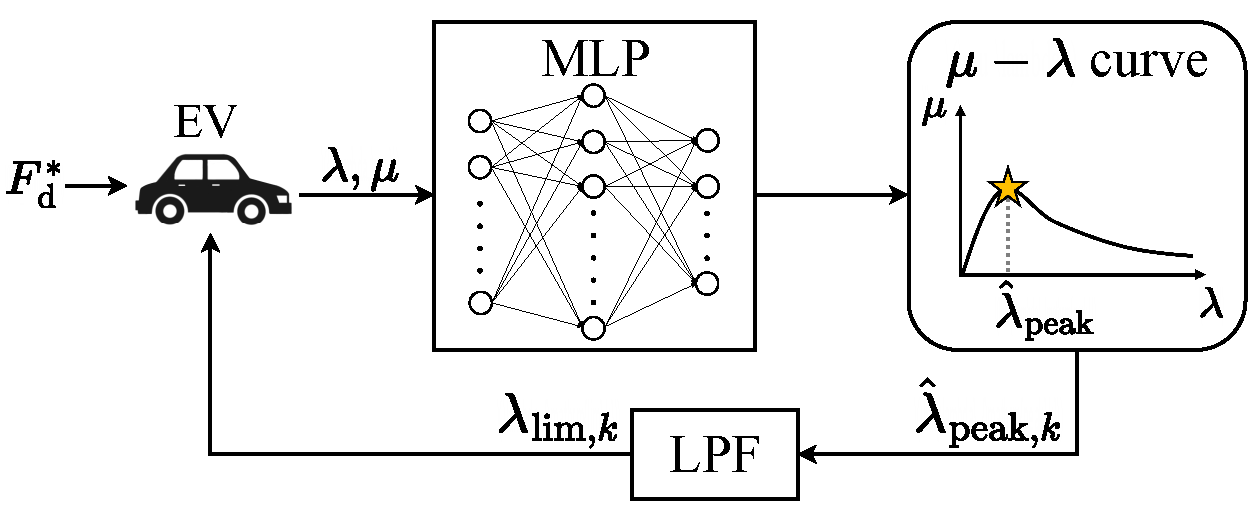
\includegraphics[width=\linewidth]{fig/1_prop_flow_simple.pdf} 
    \caption{Overview of the proposed method.}
    \label{fig:1_prop_flow_simple} 
\end{figure}


Due to their high torque response and independent wheel torque control, IWM-EVs offer advantages for vehicle motion control \cite{nam,nam2}. One of the control methods used for IWM-EVs is Driving Force Control (DFC), which controls the longitudinal driving force transmitted from the tires to the road surface \cite{yoshimura}. DFC is a type of traction control system and uses a slip ratio limiter to prevent excessive wheel slip. This allows the vehicle to follow the driving force command under normal driving conditions while suppressing excessive wheel spin on low-friction road surfaces. The driving force generated by each tire depends on the friction coefficient between the tire and road surface. The friction coefficient $\mu$ is generally expressed as a function of the slip ratio $\lambda$, and this relationship changes depending on the road surface conditions \cite{pacejka}. Therefore, the performance of DFC strongly depends on how appropriately the slip ratio limit is set.

Conventional DFC systems often use a fixed slip ratio limit determined in advance \cite{yoshimura}. To improve driving performance on various road surfaces, methods for estimating the optimal slip ratio $\lambda_\mathrm{peak}$, which corresponds to the peak friction coefficient $\mu_\mathrm{peak}$, have been studied \cite{binhminh}. However, these methods require sufficient excitation of the tire characteristics around the peak of the $\mu$--$\lambda$ curve for accurate estimation since those methods are based on recursive least squares (RLS)\cite{morimoto,maeda,mizuguchi}.  Therefore, they may not work well on road surfaces where the friction coefficient saturates without showing a clear peak \cite{sui}.

Machine-learning-based methods have also been studied. For example, neural networks have been used to directly estimate $\lambda_\mathrm{peak}$ from measured tire data \cite{crocetti}. However, these methods have mainly been evaluated through simulations. Other studies have estimated the entire $\mu$--$\lambda$ curve instead of only the optimal slip ratio \cite{mussot,berntorp,olazagoitia}. However, real-time estimation and validation through actual vehicle experiments have not been sufficiently demonstrated.

To address these issues, this paper proposes a method for estimating the optimal slip ratio by estimating the entire $\mu$--$\lambda$ curve non-parametricly in real time using a machine learning model. The proposed method estimates tire-road characteristics from partially measured data without requiring intentional slip ratio excitation or assuming a specific tire model. By using the estimated curve, an appropriate slip ratio limit can be determined even on road surfaces without a clear friction peak. An overview of the proposed estimation system is shown in Fig.~\ref{fig:1_prop_flow_simple}.

The remainder of this paper is organized as follows. Section II describes the vehicle and tire-road models. Section III presents the DFC system and the proposed estimation method. Section IV evaluates the proposed method through vehicle experiments, and Section V concludes the paper.

\section{Vehicle and Tire-Road Model}
\subsection{Vehicle Model}

The four-wheel longitudinal vehicle model used in this study is shown in Fig.~\ref{fig:2_vehicle_model}.

\begin{figure}[tb]
    \centering
    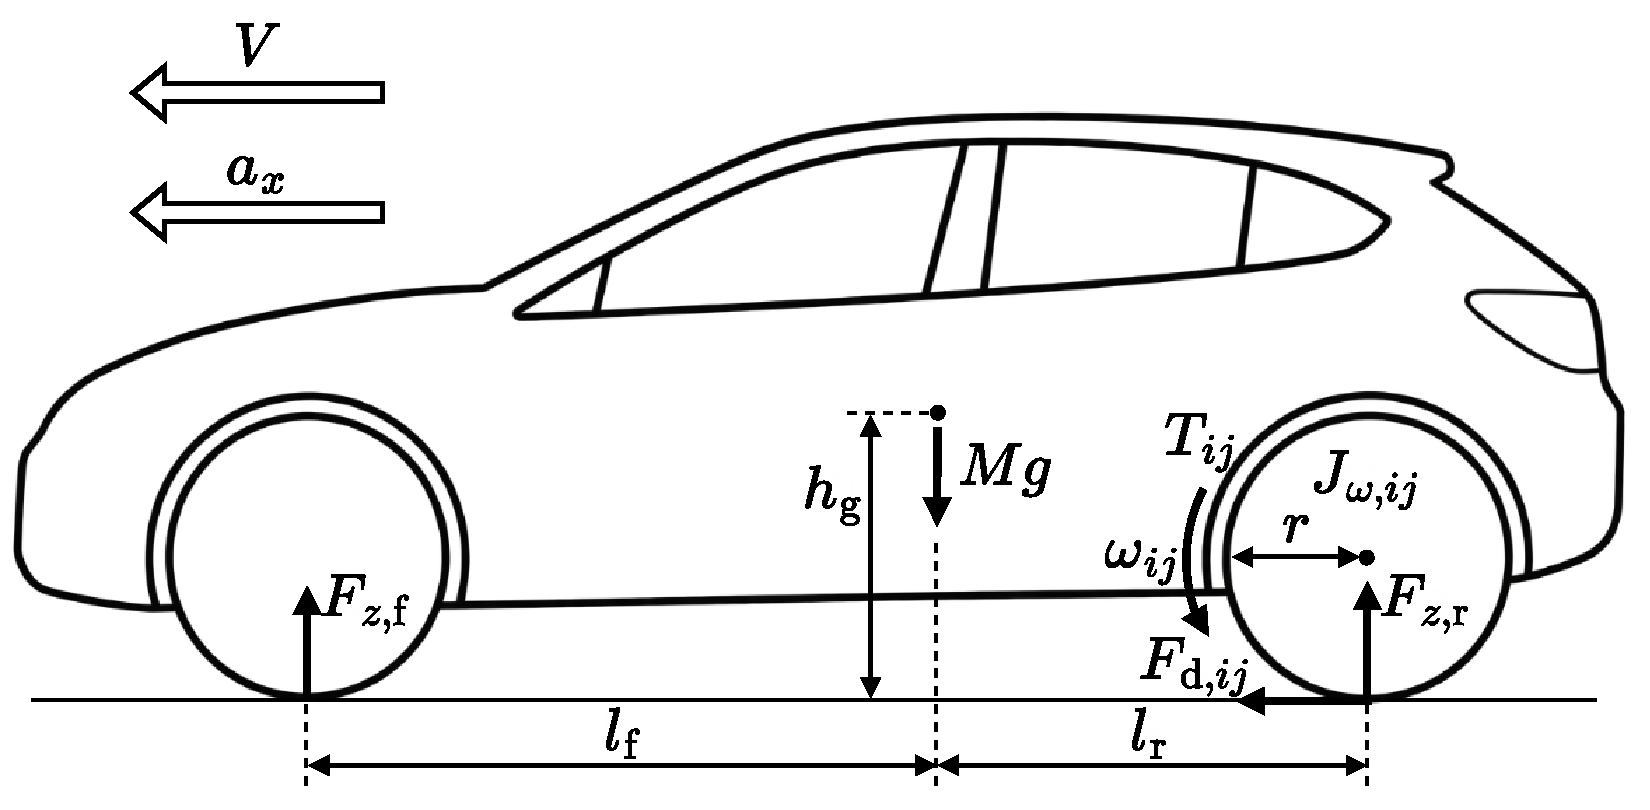
\includegraphics[width=0.8\linewidth]{fig/2_vehicle_model_4tires.pdf}
    \caption{Vehicle model.}
    \label{fig:2_vehicle_model}
\end{figure}

Neglecting driving resistance, the rotational dynamics of each wheel can be expressed as
\begin{equation}
\label{eq:2_wheel_eq}
J_{\omega,ij}\dot{\omega}_{ij}
=
T_{ij}
-
rF_{\mathrm{d},ij}
\end{equation}
where $J_{\omega,ij}$ is the wheel moment of inertia, $\omega_{ij}$ is the wheel angular velocity, $T_{ij}$ is the motor torque, $r$ is the tire radius, and $F_{\mathrm{d},ij}$ is the longitudinal driving force acting on the tireat the contact surface. The subscripts $i$ and $j$ denote the front/rear ($\mathrm{f/r}$) and left/right ($\mathrm{l/r}$) wheels, respectively.

The longitudinal motion of the vehicle is expressed as follows:
\begin{equation}
\label{eq:2_vehicle_eq}
M\dot{V}
=
F_{\mathrm{d,fl}}
+
F_{\mathrm{d,fr}}
+
F_{\mathrm{d,rl}}
+
F_{\mathrm{d,rr}}
\end{equation}
where $M$ is the vehicle mass and $V$ is the vehicle velocity.

The slip ratio of each wheel is defined by the following equation.
\begin{equation}
\label{eq:2_lambda}
\lambda_\mathrm{ij}
=
\frac{r\omega_{ij}-V}
{\max(r\omega_{ij},V,\epsilon)}
\end{equation}
where $\epsilon$ is a small positive constant introduced to prevent division by zero.

The relationship between the tire-road friction coefficient and slip ratio is shown in Fig.~\ref{fig:2_mu-lambda_curve}.
\begin{figure}[tb]
    \centering
    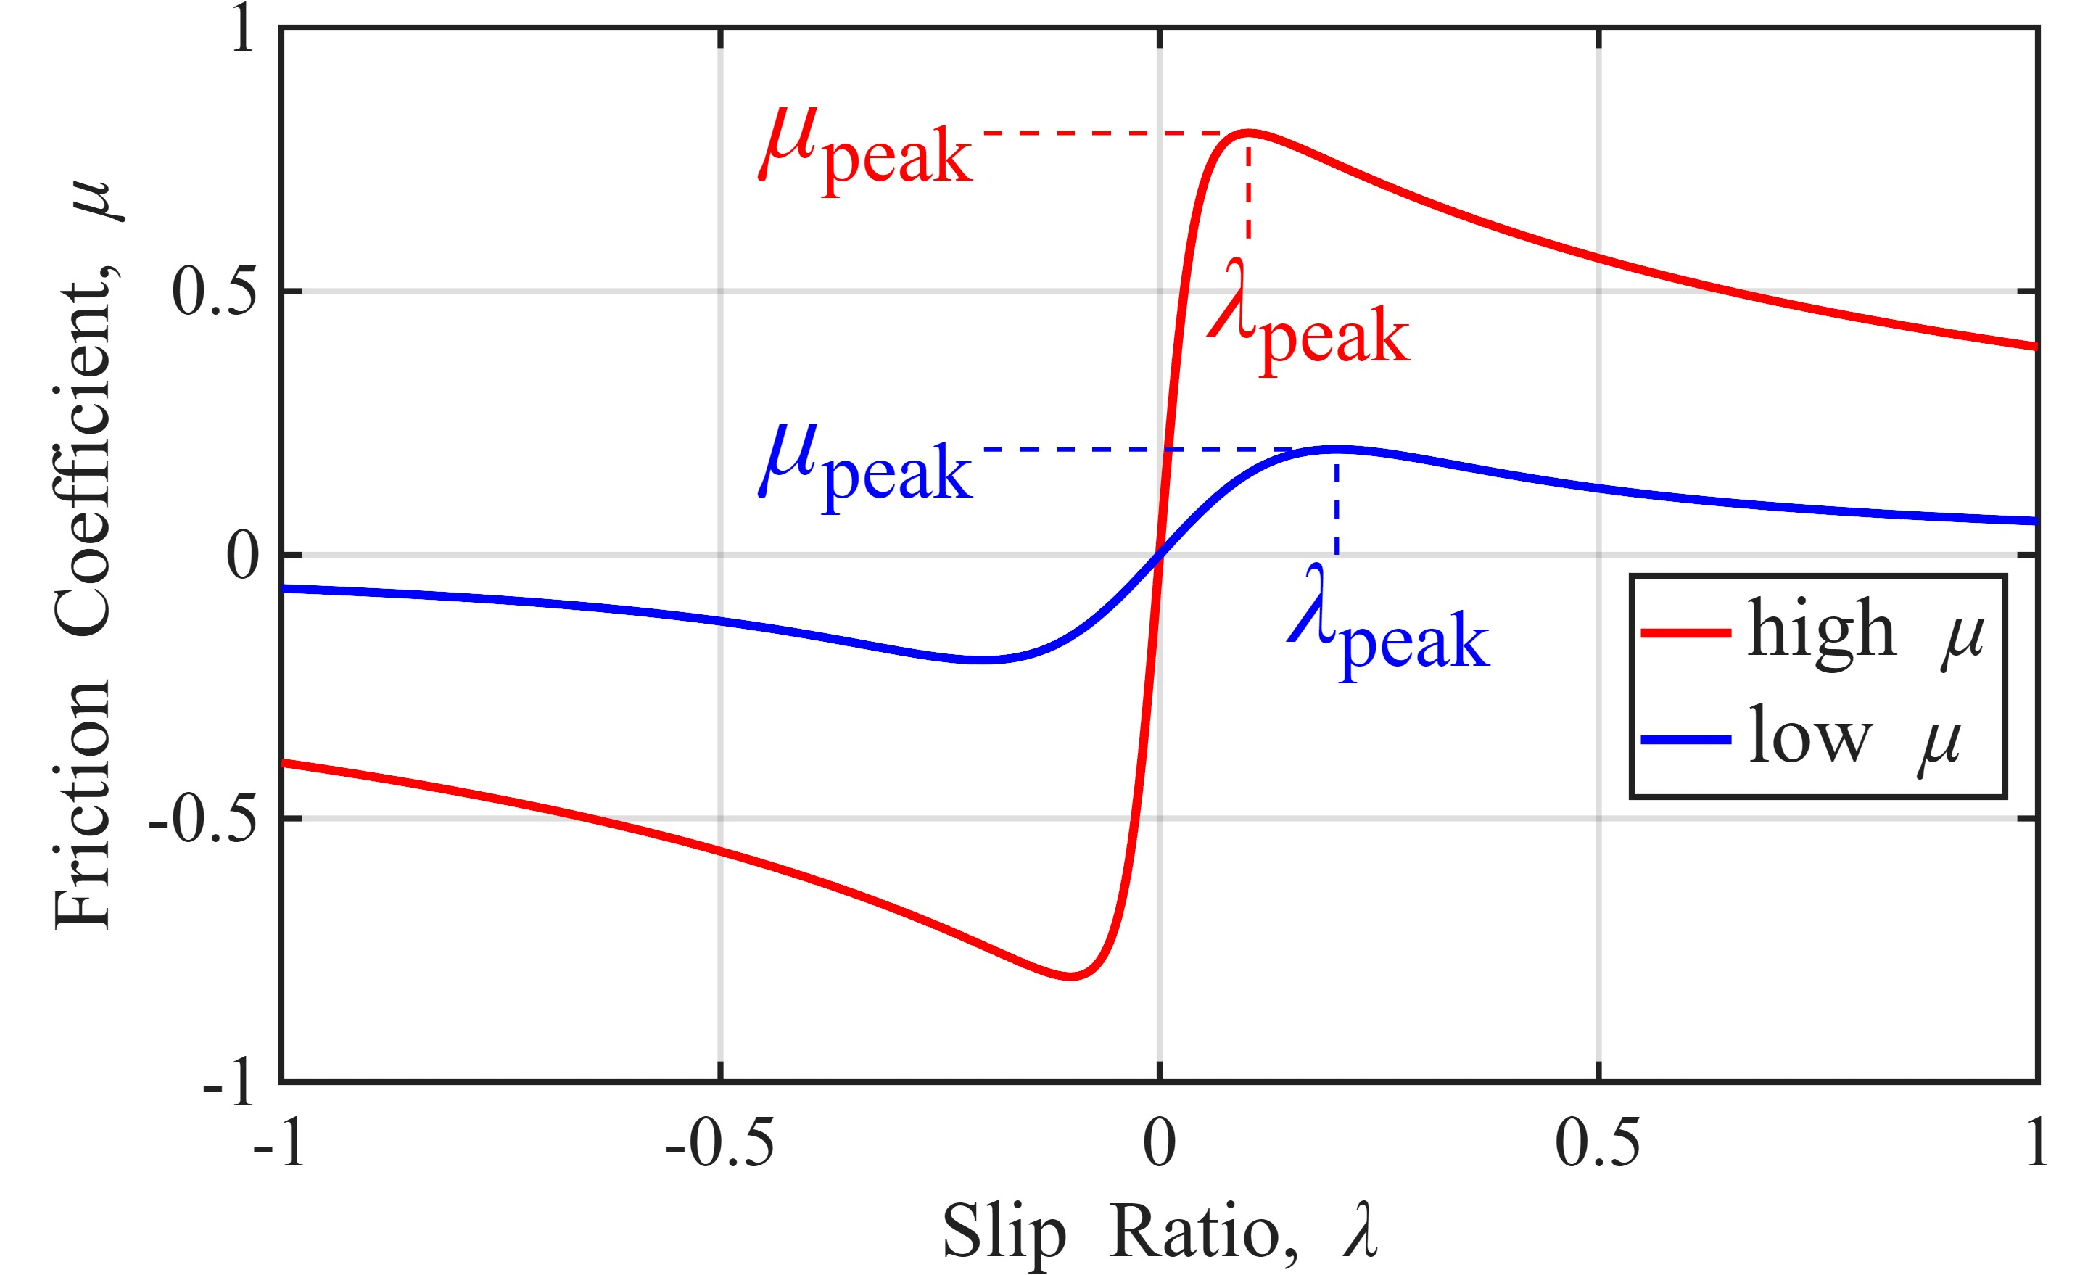
\includegraphics[width=0.6\linewidth]{fig/2_mu-lambda_curve.pdf}
    \caption{$\mu$--$\lambda$ curve.}
    \label{fig:2_mu-lambda_curve}
\end{figure}
The driving force of each wheel is given by
\begin{equation}
\label{eq:2_F_d}
F_{\mathrm{d},ij}
=
\mu_{ij}(\lambda_\mathrm{ij})
F_{\mathrm{z},ij}
\end{equation}
where $\mu_{ij}$ is the tire-road friction coefficient and $F_{\mathrm{z},ij}$ is the normal load acting on the tire. As shown in Fig.~\ref{fig:2_mu-lambda_curve}, the friction coefficient can be represented as a function of the slip ratio, and the relationship varies depending on the road surface condition \cite{pacejka}.

Considering the load transfer caused by longitudinal acceleration, the front and rear wheel loads are expressed as
\begin{equation}
\label{eq:2_F_z}
\begin{aligned}
F_{z,\mathrm{f}}
&=
\frac{l_\mathrm{r}}{2(l_\mathrm{r}+l_\mathrm{f})}Mg
-
\frac{Ma_x}{2(l_\mathrm{r}+l_\mathrm{f})}h_\mathrm{g}
\\
F_{z,\mathrm{r}}
&=
\frac{l_\mathrm{f}}{2(l_\mathrm{r}+l_\mathrm{f})}Mg
+
\frac{Ma_x}{2(l_\mathrm{r}+l_\mathrm{f})}h_\mathrm{g}
\end{aligned}
\end{equation}
where $a_x$ is the longitudinal acceleration, $l_\mathrm{f}$ and $l_\mathrm{r}$ are the distances from the center of gravity to the front and rear axles, respectively, and $h_\mathrm{g}$ is the height of the center of gravity.

\subsection{Tire-Road Model}
As shown in Fig.~\ref{fig:2_mu-lambda_curve}, the $\mu$--$\lambda$ curve exhibits highly nonlinear characteristics. One of the most widely used models for representing this relationship is the Magic Formula tire model \cite{pacejka}, which is expressed as
\begin{equation}
\label{eq:2_magicformula}
\mu_{ij}
=
D\sin\left(
C\arctan(B\lambda_{ij})
-
E\left(
B\lambda_{ij}
-
\arctan(B\lambda_{ij})
\right)
\right)
\end{equation}
where $B$, $C$, $D$, and $E$ denote the stiffness factor, shape factor, peak factor, and curvature factor, respectively. The $\mu$--$\lambda$ curve is fitted using these four coefficients.

These coefficients do not directly correspond to physical parameters but are determined through fitting to experimental tire data. Owing to its ability to accurately represent the nonlinear characteristics of tire-road friction, the Magic Formula model has been widely adopted as a standard tire model in vehicle dynamics studies.

\section{Proposed Method}
\subsection{Driving Force Control}
Driving Force Control (DFC) is widely used as a traction control method for electric vehicles \cite{yoshimura}. The block diagram of the DFC system is shown in Fig.~\ref{fig:3_DFC_circuit}.
\begin{figure}[tb]
    \centering
    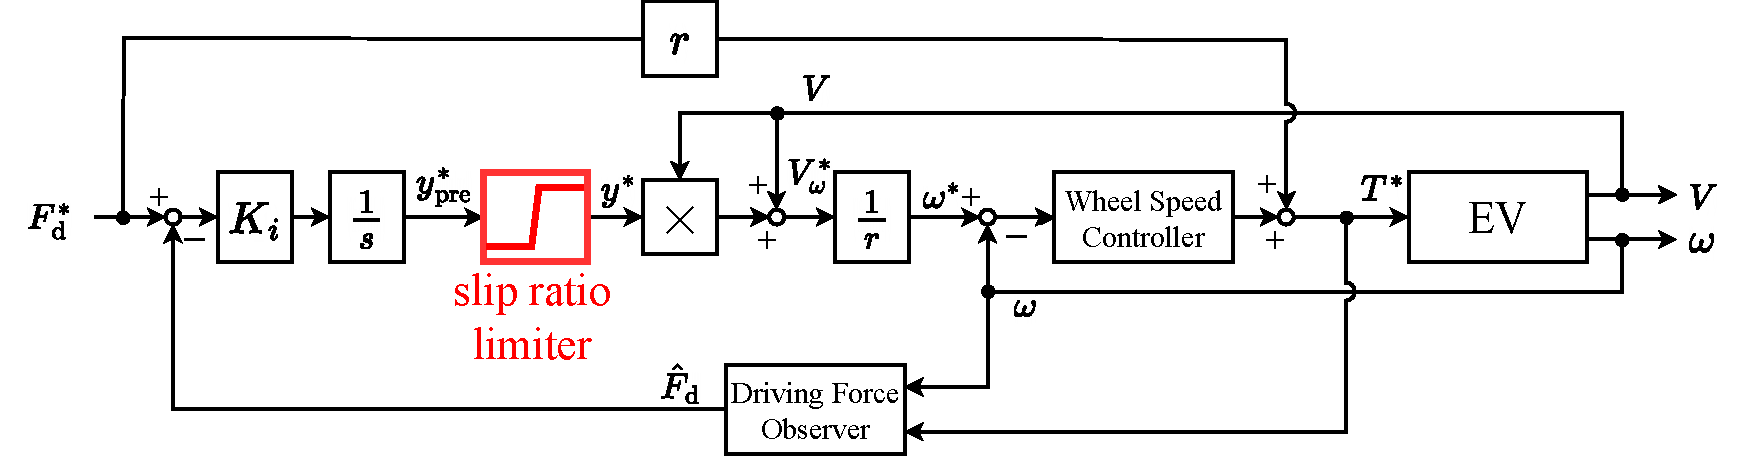
\includegraphics[width=\linewidth]{fig/3_DFC_circuit.pdf}
    \caption{Block diagram of DFC.}
    \label{fig:3_DFC_circuit}
\end{figure}

As shown in the figure, the controller has a cascade structure. The outer loop consists of a driving force control loop based on the Driving Force Observer (DFO), while the inner loop consists of a wheel speed control loop that realizes slip ratio control.The block diagram of the DFO is shown in Fig.~\ref{fig:3_DFO}.
\begin{figure}[tb]
    \centering
    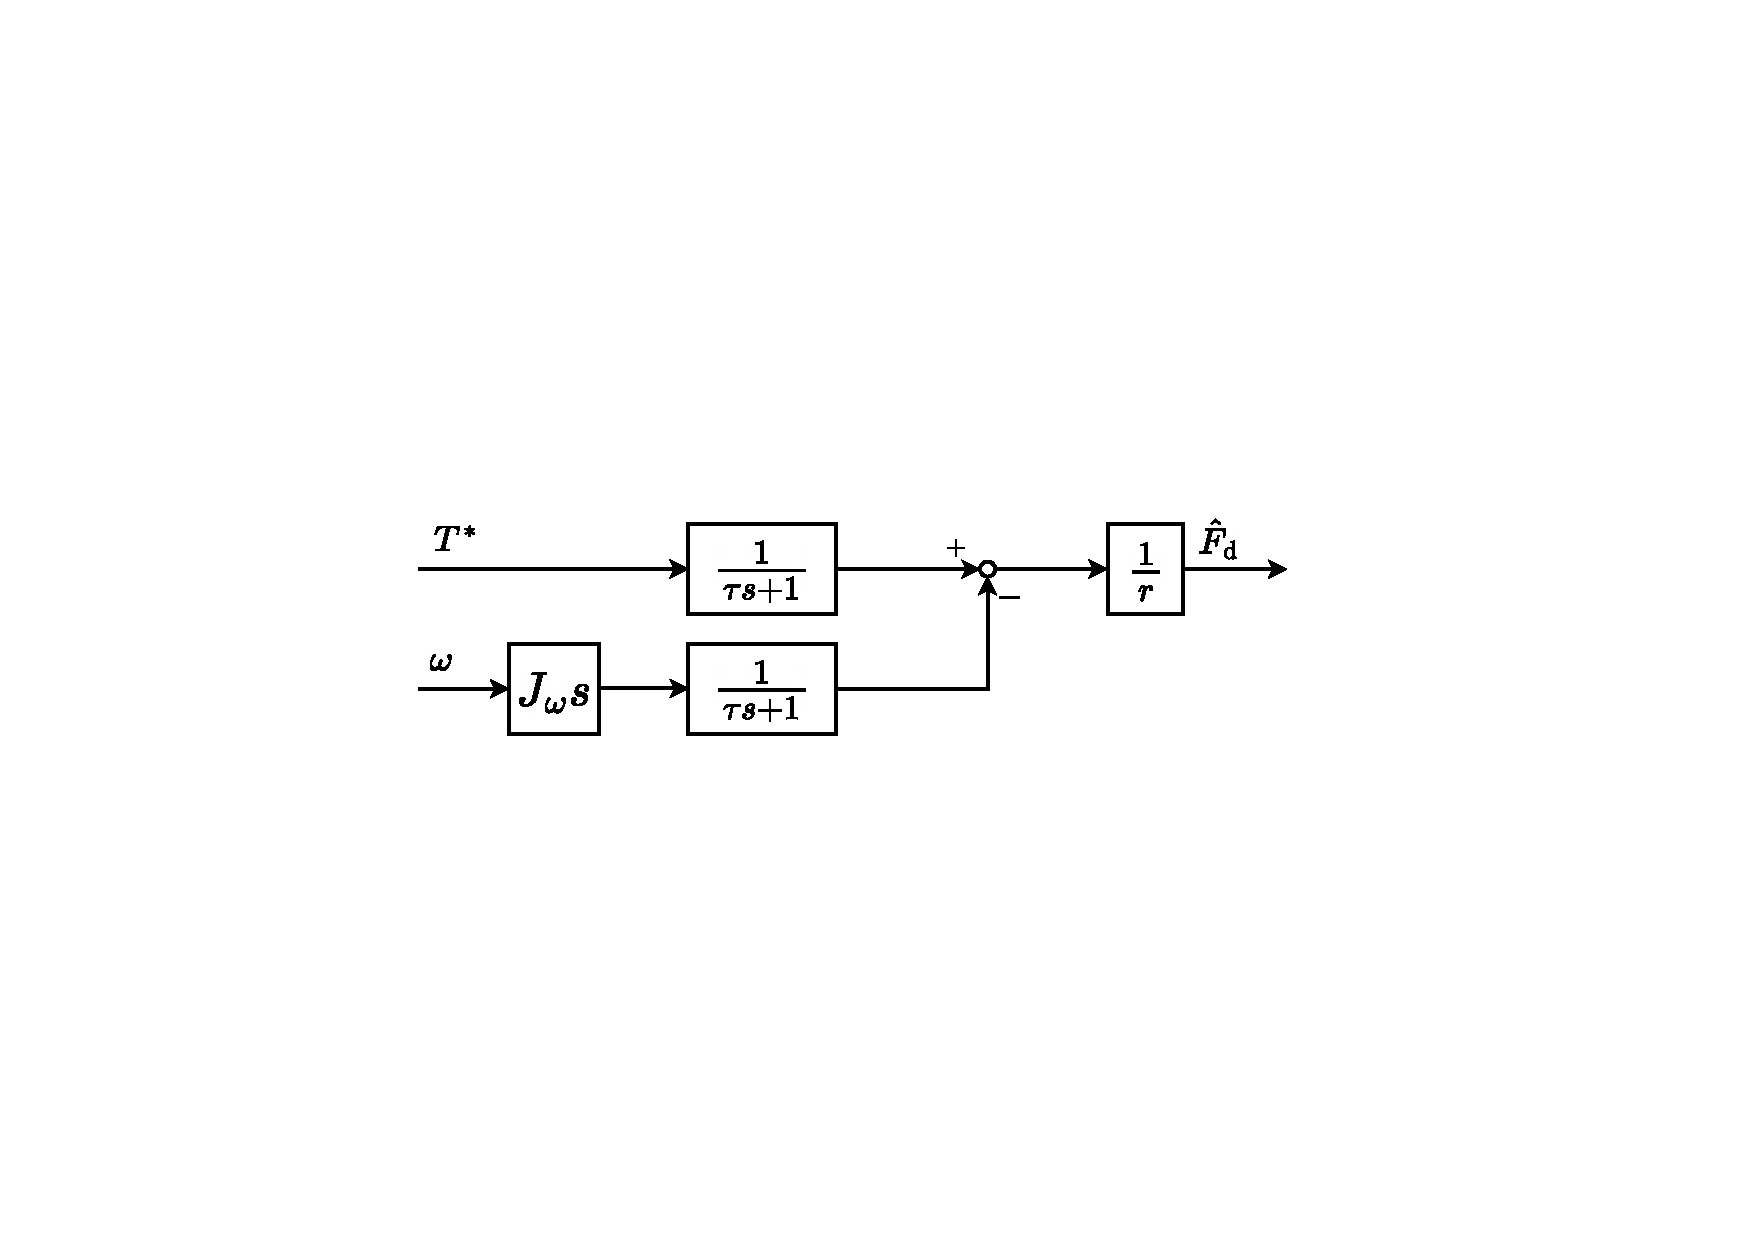
\includegraphics[width=0.8\linewidth]{fig/3_DFO.pdf}
    \caption{Driving Force Observer (DFO).}
    \label{fig:3_DFO}
\end{figure}

The estimated driving force $\hat{F}_{\mathrm{d},ij}$ is obtained as follows by rearranging (\ref{eq:2_F_d}):
\begin{equation}
\label{eq:3_DFO}
\hat{F}_{\mathrm{d},ij}
=
Q_{\mathrm{f}}(s)
\frac{
T^{*}_{ij}
-
J_{\omega,ij}\dot{\omega}_{ij}
}{r}
\end{equation}
where $Q_{\mathrm{f}}(s)=1/(\tau s+1)$ is a first-order low-pass filter with a time constant of $\tau$.

As shown in (\ref{eq:2_lambda}), the definition of slip ratio differs between driving conditions ($r\omega_{ij}\geq V$) and braking conditions ($r\omega_{ij}<V$), which is inconvenient for control design. Therefore, instead of directly controlling the slip ratio, the following control variable $y_{ij}$ is introduced:
\begin{equation}
\label{eq:3_y}
y_{ij}
=
\frac{r\omega_{ij}-V}{V}
=
\frac{r\omega_{ij}}{V}-1
\end{equation}

The variable $y_{ij}$ is equivalent to the slip ratio under braking conditions, and in the low-slip region, $y_{ij}$ and $\lambda_{ij}$ take almost identical values. The reference value $y^{*}$ is generated through integral control of the driving force command.

On low-friction road surfaces with a small peak friction coefficient $\mu_{\mathrm{peak}}$, the physically achievable maximum driving force $F_{\mathrm{d,max}}(=\mu_{\mathrm{peak}}F_{z})$ may become smaller than the driving force command $F_{\mathrm{d}}^{*}$. In such situations, excessive wheel slip may occur. Therefore, a slip ratio limiter is introduced to generate traction performance by restricting wheel slip.

As shown in Fig.~\ref{fig:2_mu-lambda_curve}, by setting the slip ratio limiter to the optimal slip ratio $\lambda_{\mathrm{peak}}$, at which the friction coefficient reaches its maximum value (or saturation), both traction performance and maximum driving force utilization can be achieved simultaneously.

\subsection{Overview of the Proposed $\lambda_{\mathrm{peak}}$ Estimation Method}

In this study, the entire $\mu$--$\lambda$ curve is estimated from the observed $(\mu,\lambda)$ data during driving, and the optimal slip ratio $\lambda_{\mathrm{peak}}$ is obtained from the estimated curve. A detailed block diagram of the proposed method is shown in Fig.~\ref{fig:3_prop_flow_detail}.

\begin{figure*}[tb]
    \centering
    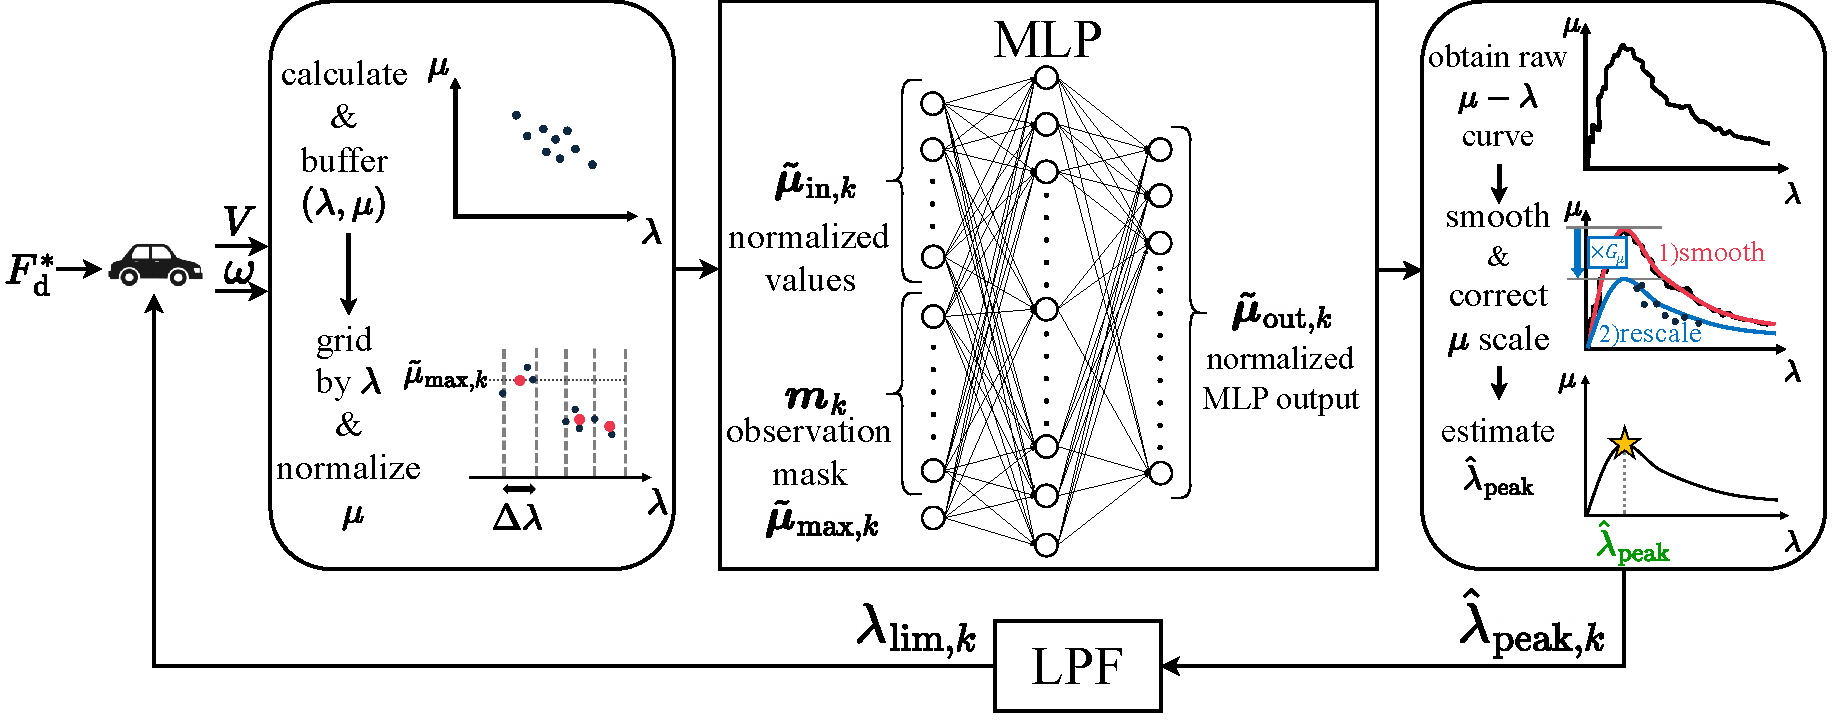
\includegraphics[width=0.6\textwidth]{fig/prop_flow_detail.pdf}
    \caption{Detailed block diagram of the proposed method.}
    \label{fig:3_prop_flow_detail}
\end{figure*}

A Multi-Layer Perceptron (MLP) is employed to estimate the entire shape of the $\mu$--$\lambda$ curve. The trained MLP generates the estimated $\mu$--$\lambda$ curve in real time from sequentially measured $\mu$ and $\lambda$ values.

\subsection{MLP-Based $\mu$--$\lambda$ Curve Estimation}

\subsubsection{MLP Architecture and Training Conditions}

To estimate the $\mu$--$\lambda$ curve, a fully connected MLP with three hidden layers was employed. As described later, the dimensions of the input and output layers were set to $2n+1$ and $n$, respectively, and each hidden layer consisted of 128 neurons.

The ReLU activation function was used in the hidden layers, while a linear activation function was adopted for the output layer. Adam \cite{kingma} was used as the optimization algorithm. The learning rate, mini-batch size, and number of training epochs were set to $1.0\times10^{-4}$, 1024, and 1000, respectively.

\subsubsection{MLP Inputs}

First, the slip ratio $\lambda_{ij}$ and friction coefficient $\mu$ are calculated from the measured wheel angular velocity $\omega_{ij}$ and vehicle velocity $V$, and the latest 200 samples are stored in a buffer. The slip ratio is calculated using (\ref{eq:2_lambda}), and the friction coefficient is calculated from the DFO output $\hat{F}_{\mathrm{d},ij}$ and the estimated normal load $\hat{F}_{z,ij}$ using (\ref{eq:2_F_d}). The estimated normal load $\hat{F}_{z,ij}$ is obtained from $a_x$ using (\ref{eq:2_F_z}).

Next, the buffered $(\lambda,\mu)$ data are discretized into grids with a constant interval of $\Delta\lambda=0.001$. The average value of $\mu$ within each grid is used as the representative point of that grid. This procedure fixes the input dimension of the MLP.

Furthermore, all representative points are normalized by the maximum friction coefficient among the representative points, denoted by $\tilde{\mu}_{\mathrm{max}}$. This normalization reduces the influence of the friction scale and improves the generalization capability of the model for various road surfaces.

Finally, the input vector at time step $k$ consists of the normalized friction vector $\boldsymbol{\tilde{\mu}}_{\mathrm{in},k}$, a binary mask vector $\boldsymbol{m}_k$ indicating whether each grid contains measured points, and $\tilde{\mu}_{\mathrm{max},k}$, resulting in a $(2n+1)$-dimensional input vector.

In this study, the target slip ratio range was selected as $0\le\lambda\le0.5$ considering practical driving conditions, and the number of grids was set to $n=501$.

\subsubsection{MLP Training}

\begin{figure}[tb]
    \centering
    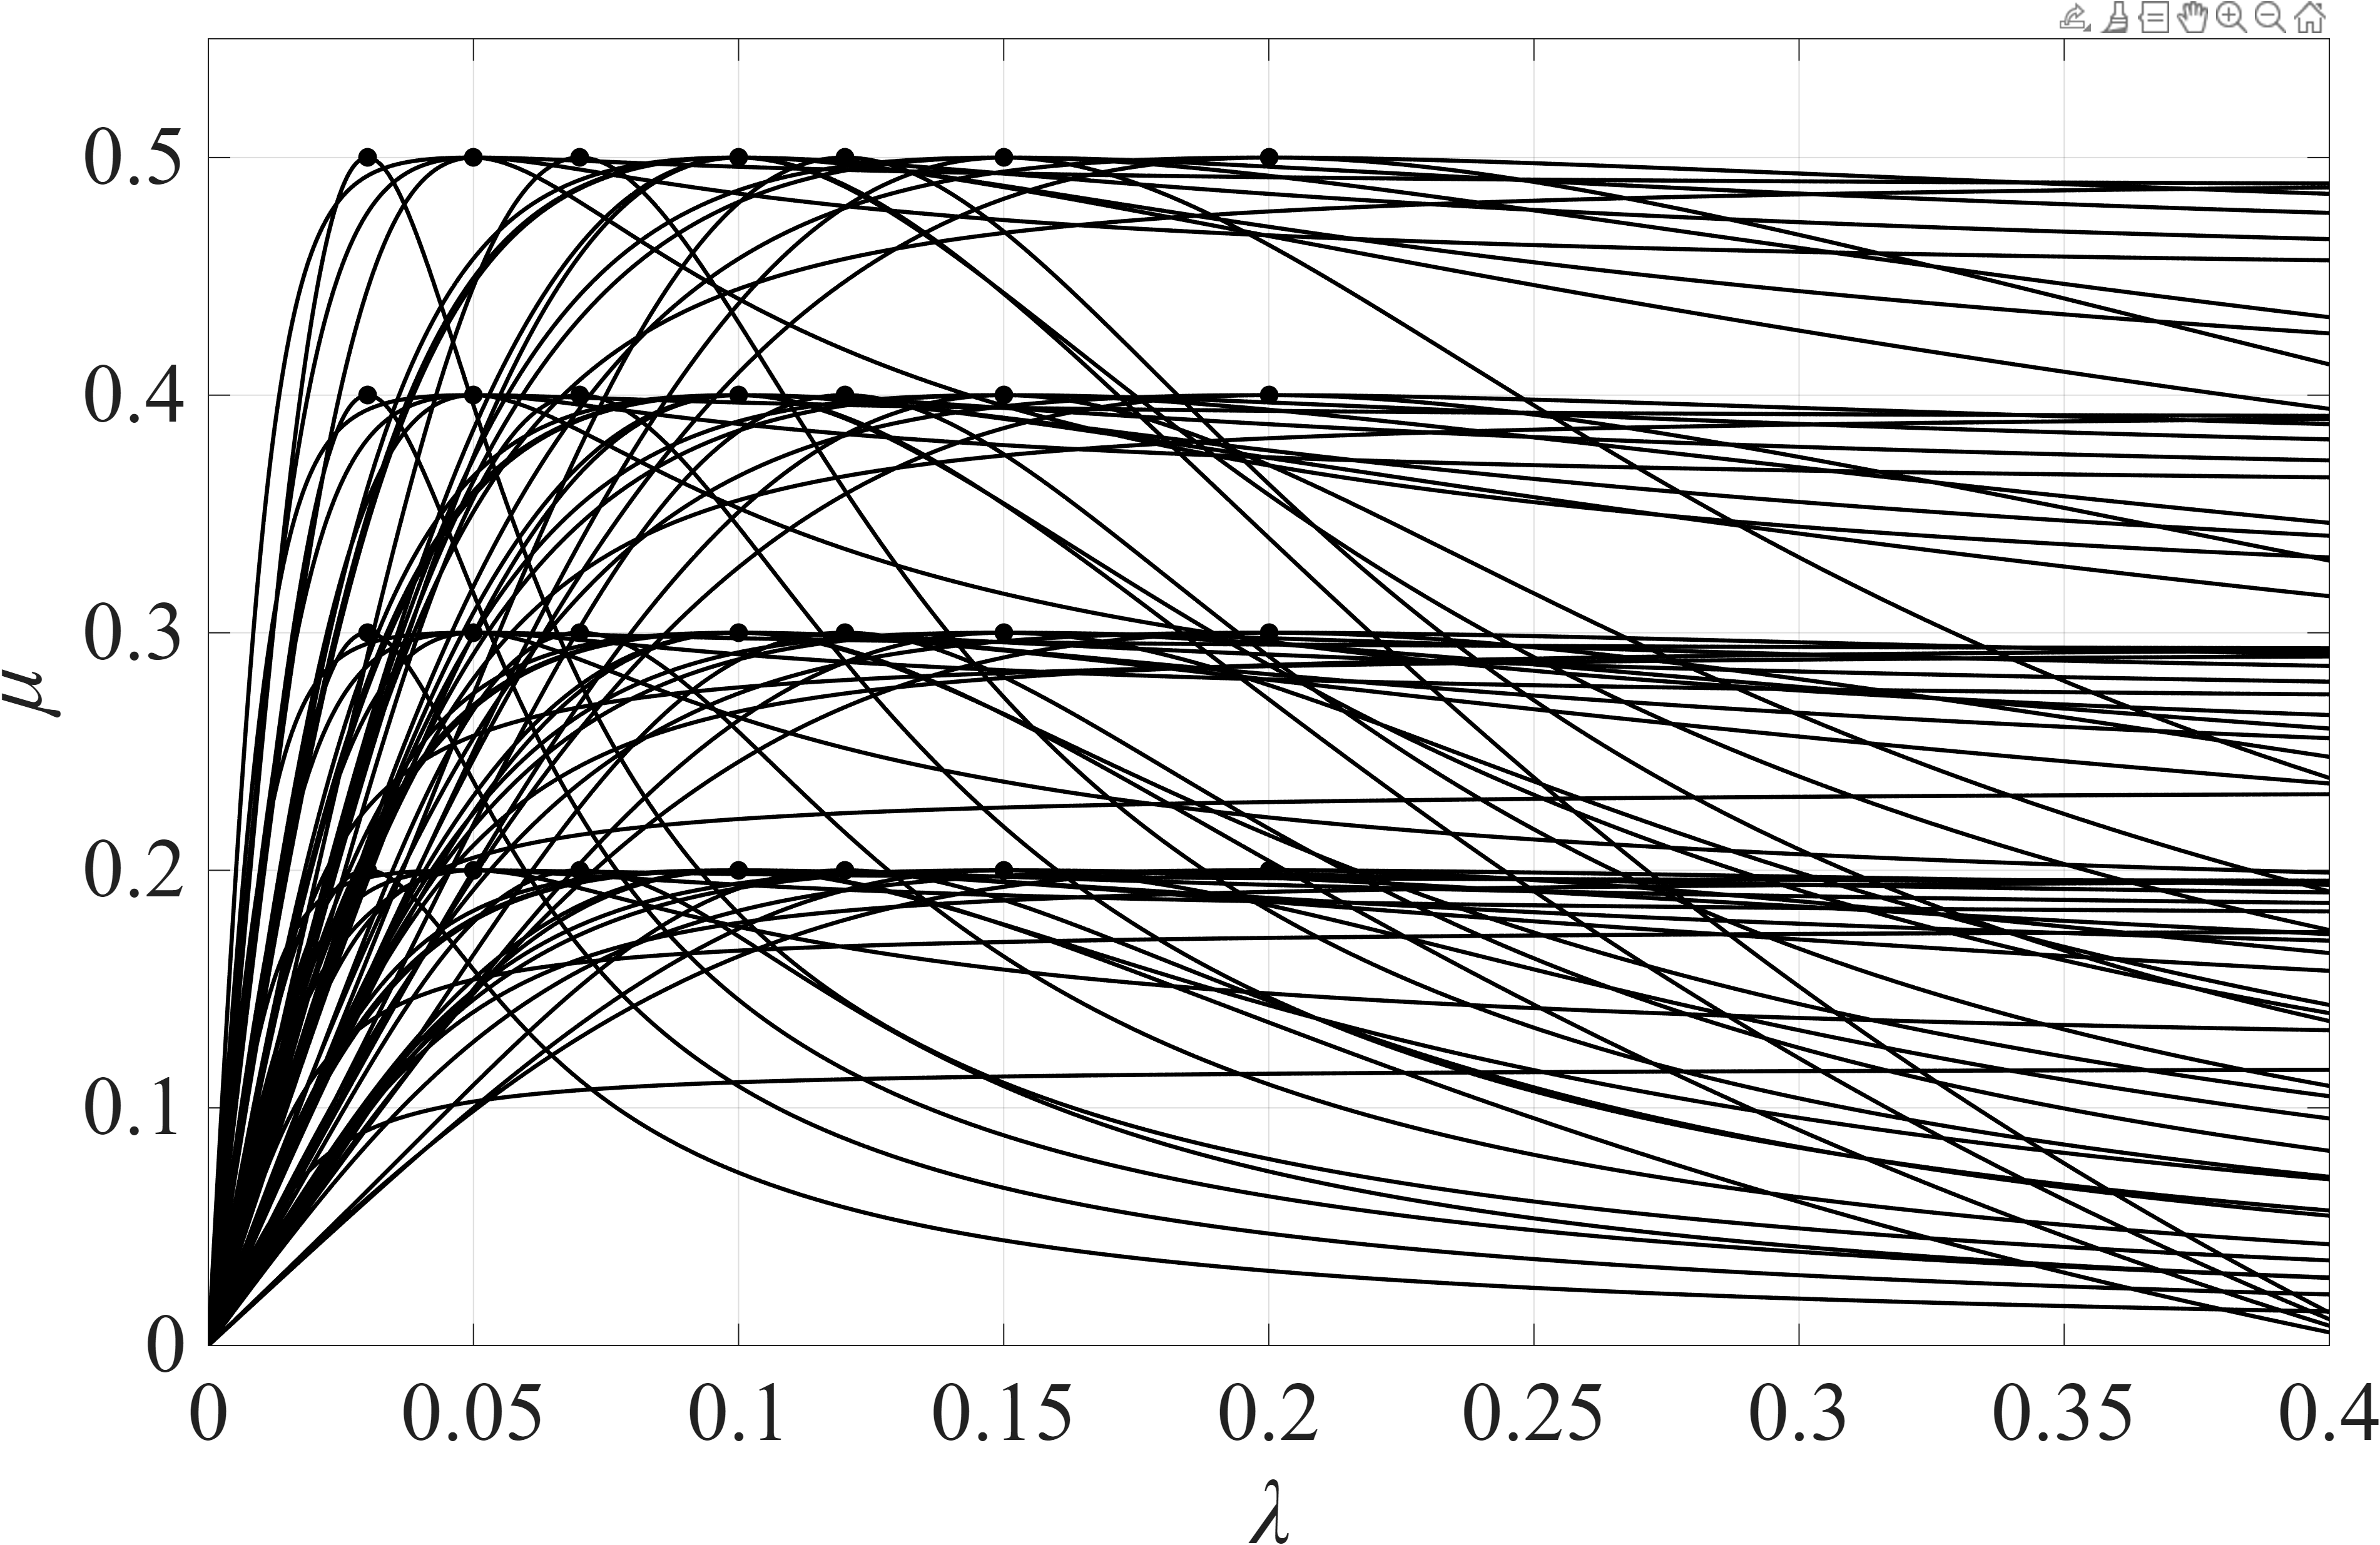
\includegraphics[width=0.7\linewidth]{fig/3_magic_formula_curves.png}
    \caption{Training $\mu$--$\lambda$ curves.}
    \label{fig:3_magic_formula_curve}
\end{figure}

The training data were generated using MATLAB/Simulink. The Magic Formula model described previously was used to generate the teacher curves. To prevent the shape of the curve from being uniquely determined by the peak friction coefficient, various curve shapes were generated while fixing the coefficient $D$ that defines $\mu_{\mathrm{peak}}$. Subsequently, the coefficient $D$ was varied among 0.2, 0.3, 0.4, and 0.5, resulting in a total of 72 road surface models.
The generated training curves are shown in Fig.~\ref{fig:3_magic_formula_curve}.
Simulation results representing vehicle driving on each road surface were used to generate the training inputs. Since only partial $\mu$--$\lambda$ observations are available during actual driving, partial observations must also be reproduced during training.

Therefore, slip ratio control was performed in simulation using a triangular-wave slip-ratio command over the range $0\le\lambda\le0.6$ to obtain sufficiently wide $\mu$--$\lambda$ characteristics. Random observation ranges were then generated using random seeds to reproduce realistic partial measurements.

The loss function used for MLP training is defined as
\begin{equation}
\label{eq:3_L_total}
L_{\mathrm{Total}}
=
0.1L_{\mathrm{Data}}
+
1.0L_{\mathrm{Input}}
\end{equation}
where $L_{\mathrm{Data}}$ and $L_{\mathrm{Input}}$ are the mean squared errors (MSEs) with respect to the teacher data and the input observations, respectively. Both losses are calculated using grid-averaged values. For $L_{\mathrm{Input}}$, only grids containing measured points are considered.

By assigning a sufficiently larger weight to $L_{\mathrm{Input}}$ than to $L_{\mathrm{Data}}$, the network is encouraged to accurately reproduce observed points while generating physically reasonable extrapolations in unobserved regions based on the learned training data.

\subsubsection{MLP Outputs}
\begin{figure}[tb]
    \centering
    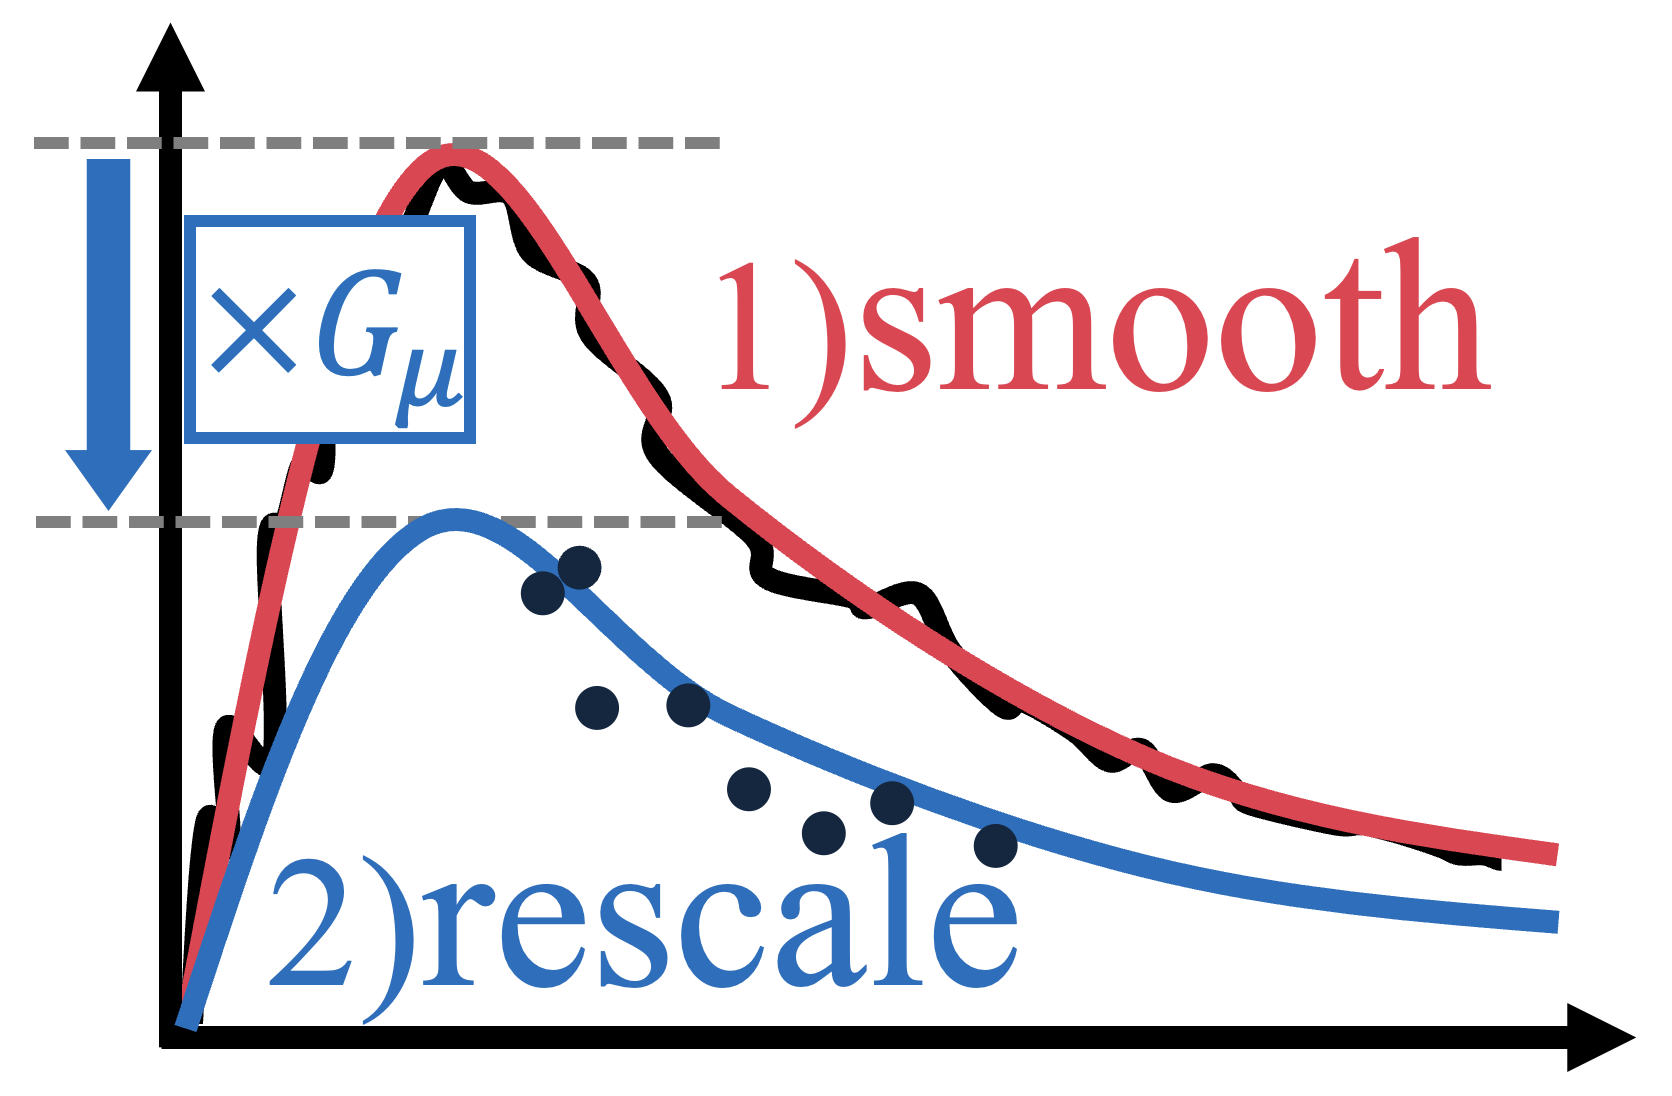
\includegraphics[width=0.5\linewidth]{fig/3_filter_rescale.png}
    \caption{Smoothing and rescaling of the MLP output.}
    \label{fig:3_filter_rescale}
\end{figure}

The MLP outputs an $n$-dimensional vector
$\boldsymbol{\tilde{\mu}}_{\mathrm{out},k}$,
which consists of normalized estimates of the friction coefficient
at each slip-ratio grid point.

Since the MLP estimates each grid value independently, oscillations may appear in the output on the $\mu$--$\lambda$ plane. In addition, the output remains normalized and therefore requires the post-processing shown in Fig.~\ref{fig:3_filter_rescale}.

First, a Savitzky-Golay filter \cite{SGfilter} with a polynomial order of 3 and a window length of 51 is applied to suppress oscillations.

Next, the normalized output is rescaled to match the magnitude of the observed friction coefficients. The scaling gain $G_{\mu,k}$ is obtained by minimizing the squared error between the scaled MLP output and the unnormalized inputs, as follows:
\begin{equation}
\label{eq:G_mu}
G_{\mu,k}
=
\frac{
\displaystyle
\sum_{i:m_{i,k}=1}
\tilde{\mu}_{\mathrm{out},i,k}
\mu_{\mathrm{in},i,k}
}{
\displaystyle
\sum_{i:m_{i,k}=1}
\tilde{\mu}_{\mathrm{out},i,k}^{2}
}
\end{equation}
where $i\in\{1,\ldots,n\}$ denotes the grid index and $m_{i,k}=1$ indicates the presence of observations in Grid $i$ at time step~$k$.

Through the above procedures, the $\mu$--$\lambda$ curve can be estimated online in a non-parametric manner.

\subsection{$\lambda_{\mathrm{peak}}$ Estimation}

\begin{figure}[tb]
    \centering
    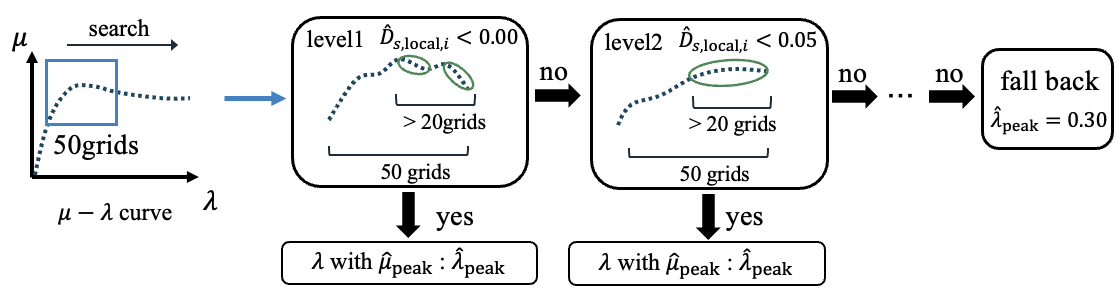
\includegraphics[width=\linewidth]{fig/3_estimate_peak.png}
    \caption{$\hat{\lambda}_{\mathrm{peak}}$ estimation algorithm.}
    \label{fig:3_estimate_peak}
\end{figure}

The optimal slip ratio is estimated from the estimated $\mu$--$\lambda$ curve. The flowchart of the algorithm is shown in Fig.~\ref{fig:3_estimate_peak}.

First, the local gradient of the estimated $\mu$--$\lambda$ curve is calculated as
\begin{equation}
\label{eq:3_D_s}
\hat{D}_{\mathrm{s,local},i}
=
\frac{\mu_{i+1}-\mu_{i-1}}
{2\Delta\lambda}
\end{equation}
where $\Delta\lambda$ denotes the grid interval. At the boundaries, one-sided differences are used instead of central differences.

Next, among all consecutive sets of 50 grids, the set with the smallest slip ratio containing at least 20 grids satisfying $\hat{D}_{\mathrm{s,local},i}<0$ is selected. Within this set, the maximum friction coefficient is defined as the estimated peak friction coefficient $\hat{\mu}_{\mathrm{peak}}$, and the corresponding slip ratio is defined as the estimated optimal slip ratio $\hat{\lambda}_{\mathrm{peak}}$.

If no such set exists, the threshold is relaxed to $\hat{D}_{\mathrm{s,local},i}<0.05$, followed by the same search process. If no valid set is found, the threshold is further relaxed to $\hat{D}_{\mathrm{s,local},i}<0.10$. If a valid set still cannot be found, the estimation is terminated and $\hat{\lambda}_{\mathrm{peak}}=0.30$ is assigned.

This procedure enables estimation of the slip ratio corresponding to friction saturation even when the $\mu$--$\lambda$ curve does not exhibit a distinct peak. In addition, robust peak detection can be achieved even when residual oscillations remain in the estimated curve.

\subsubsection{Setting of $\lambda_{\mathrm{lim}}$}
The estimated $\hat{\lambda}_{\mathrm{peak}}$ may change rapidly, causing the slip-ratio command to fluctuate and possibly making the vehicle unstable on low-friction surfaces. Therefore, a low-pass filter is used to reduce these fluctuations.

Furthermore, DFC uses the control variable $y$ instead of the slip ratio $\lambda$, as described previously. Therefore, the slip-ratio limit $\lambda_{\mathrm{lim}}$ must be converted into the control input limit $y_{\mathrm{lim}}$ according to
\begin{equation}
\label{eq:3_y_lim}
y_{\mathrm{lim}}
=
\frac{\lambda_{\mathrm{lim}}}
{1-\lambda_{\mathrm{lim}}}
\end{equation}

\section{Experimental Validation of the Proposed Method}

\subsection{Experimental Vehicle}
\begin{figure}[tb]
    \centering
    \subfloat[FPEV-2 Kanon]{
        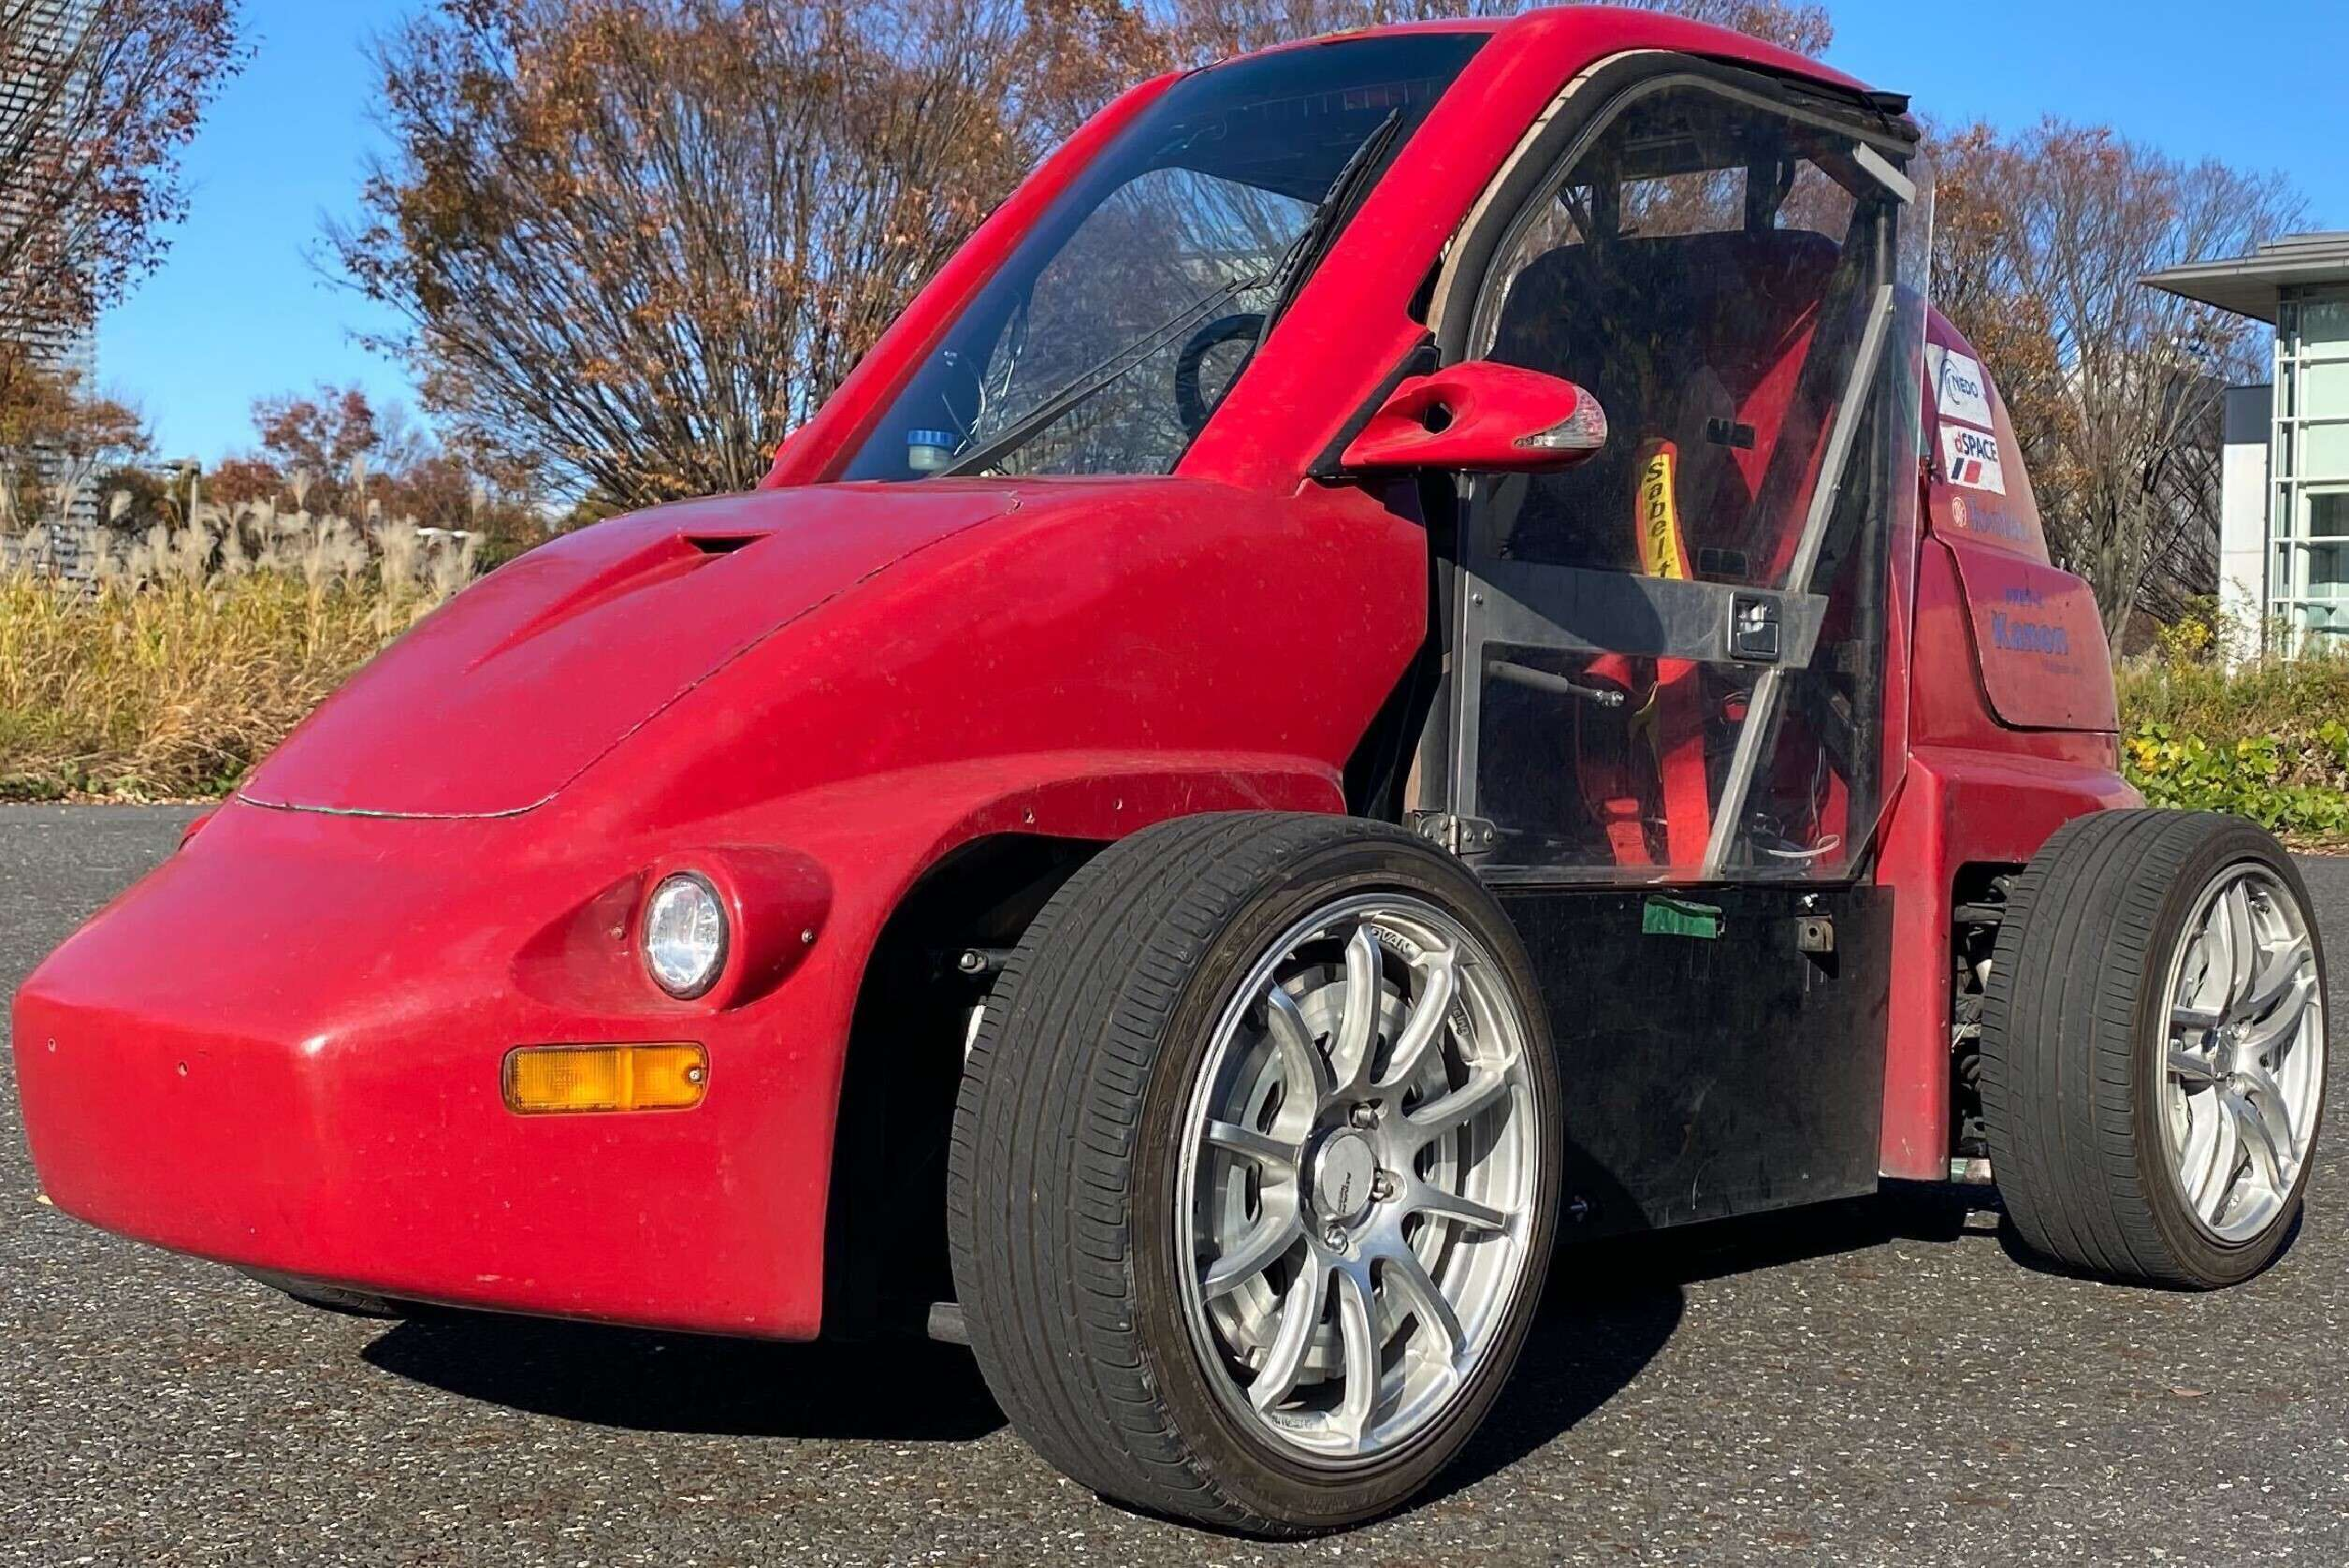
\includegraphics[height=2.7cm]{fig/2_Kanon.pdf}
        \label{subfig:2_Kanon}
    }
    \hfill
    \subfloat[In-wheel motor]{
        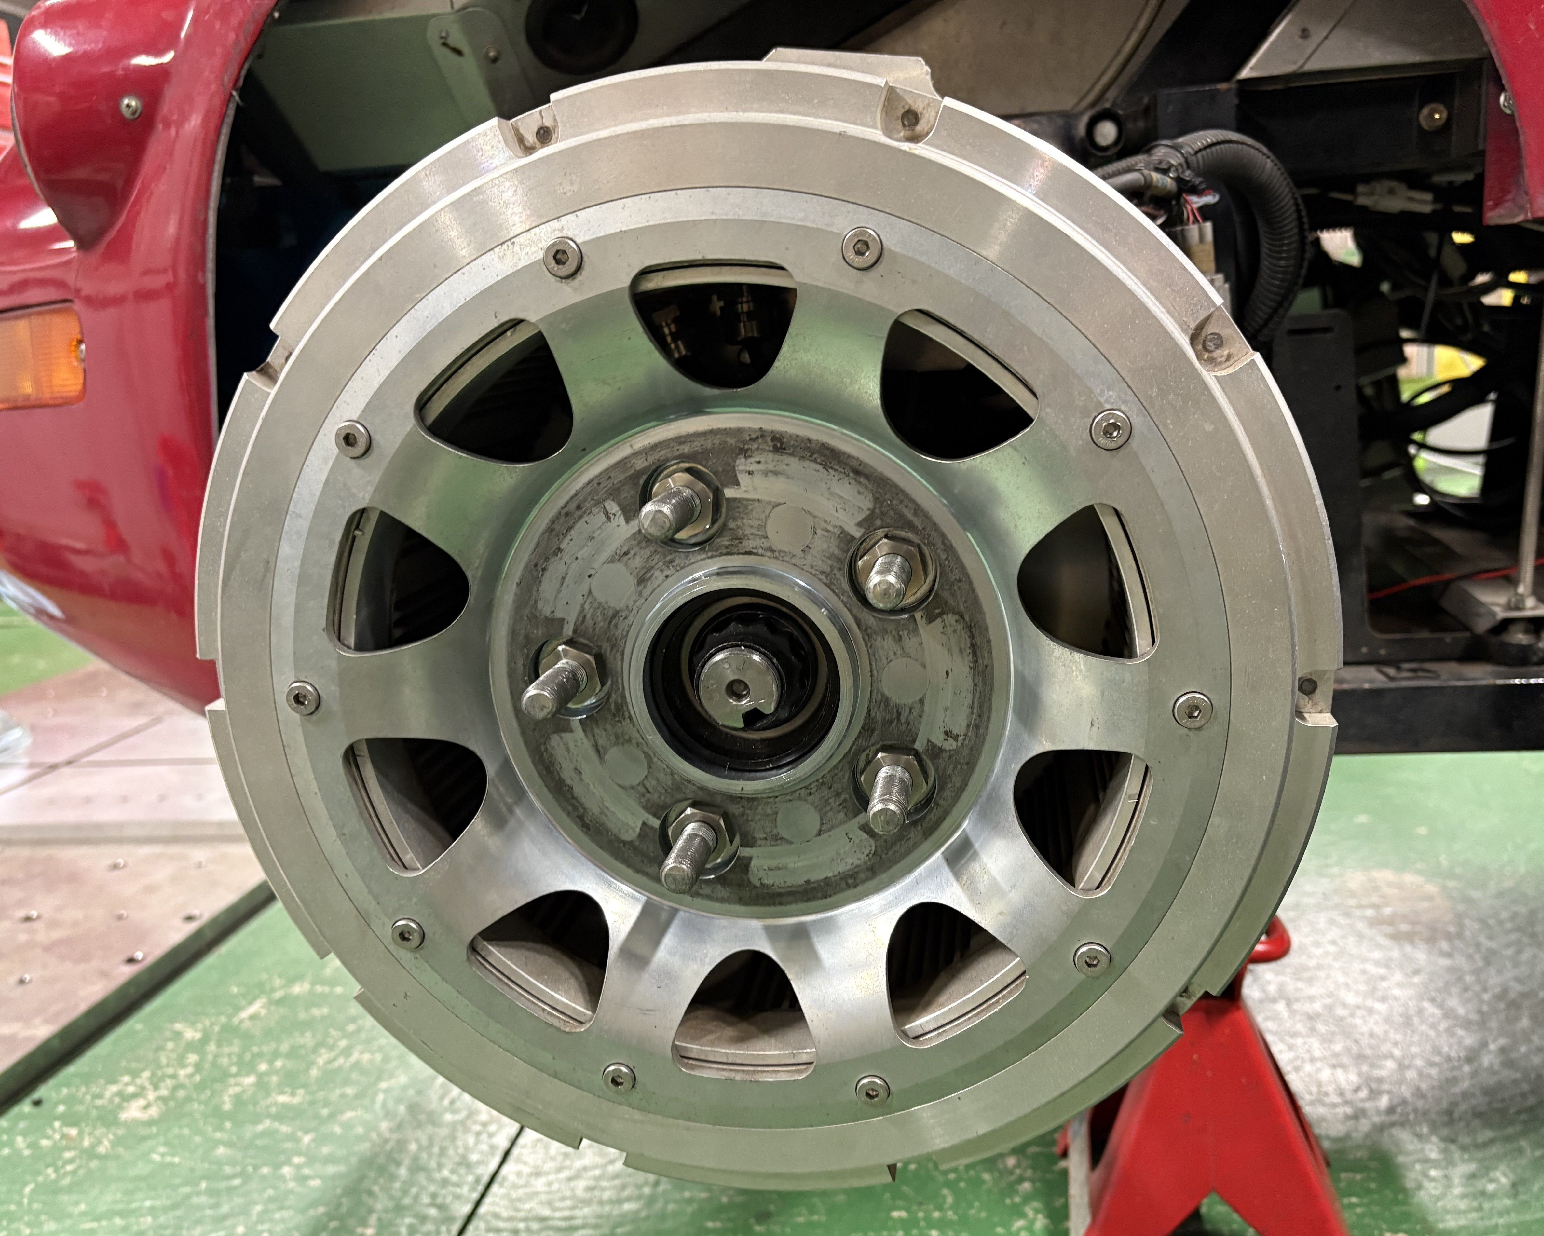
\includegraphics[height=2.7cm]{fig/2_Kanon_front_IWM.pdf}
        \label{subfig:2_IWM}
    }
    \caption{Experimental vehicle and in-wheel motor.}
    \label{fig:2_Kanon_IWM}
\end{figure}

The four-wheel in-wheel-motor electric vehicle (IWM-EV), FPEV-2 Kanon, developed by the authors' research group, was used as the experimental vehicle, as shown in Fig.~\ref{subfig:2_Kanon}.
The in-wheel motor (IWM) installed in the vehicle is shown in Fig.~\ref{subfig:2_IWM}.


\subsection{Experimental Conditions}

\begin{figure}[tb]
    \centering
    \subfloat[Experimental road surface setup]{
        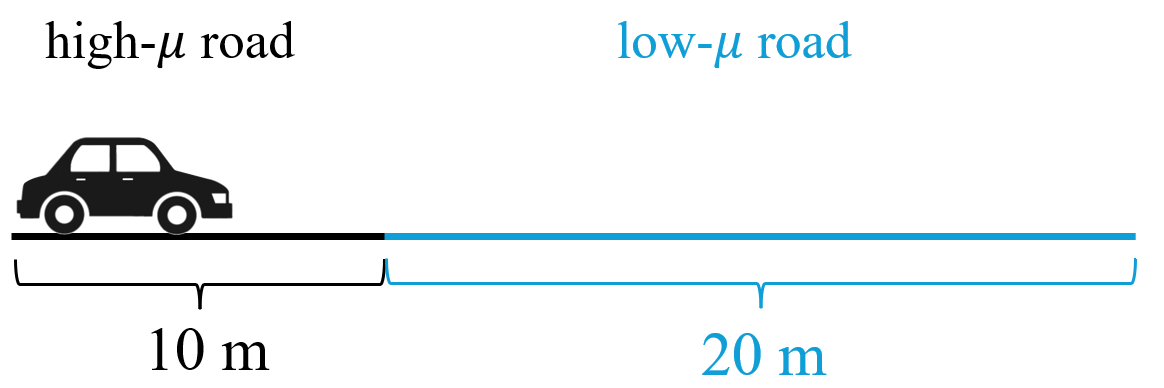
\includegraphics[width=0.68\linewidth]{fig/4_road_condition.png}
        \label{subfig:4_road_condition}
    }
    \hfill
    \subfloat[Composite sheet]{
        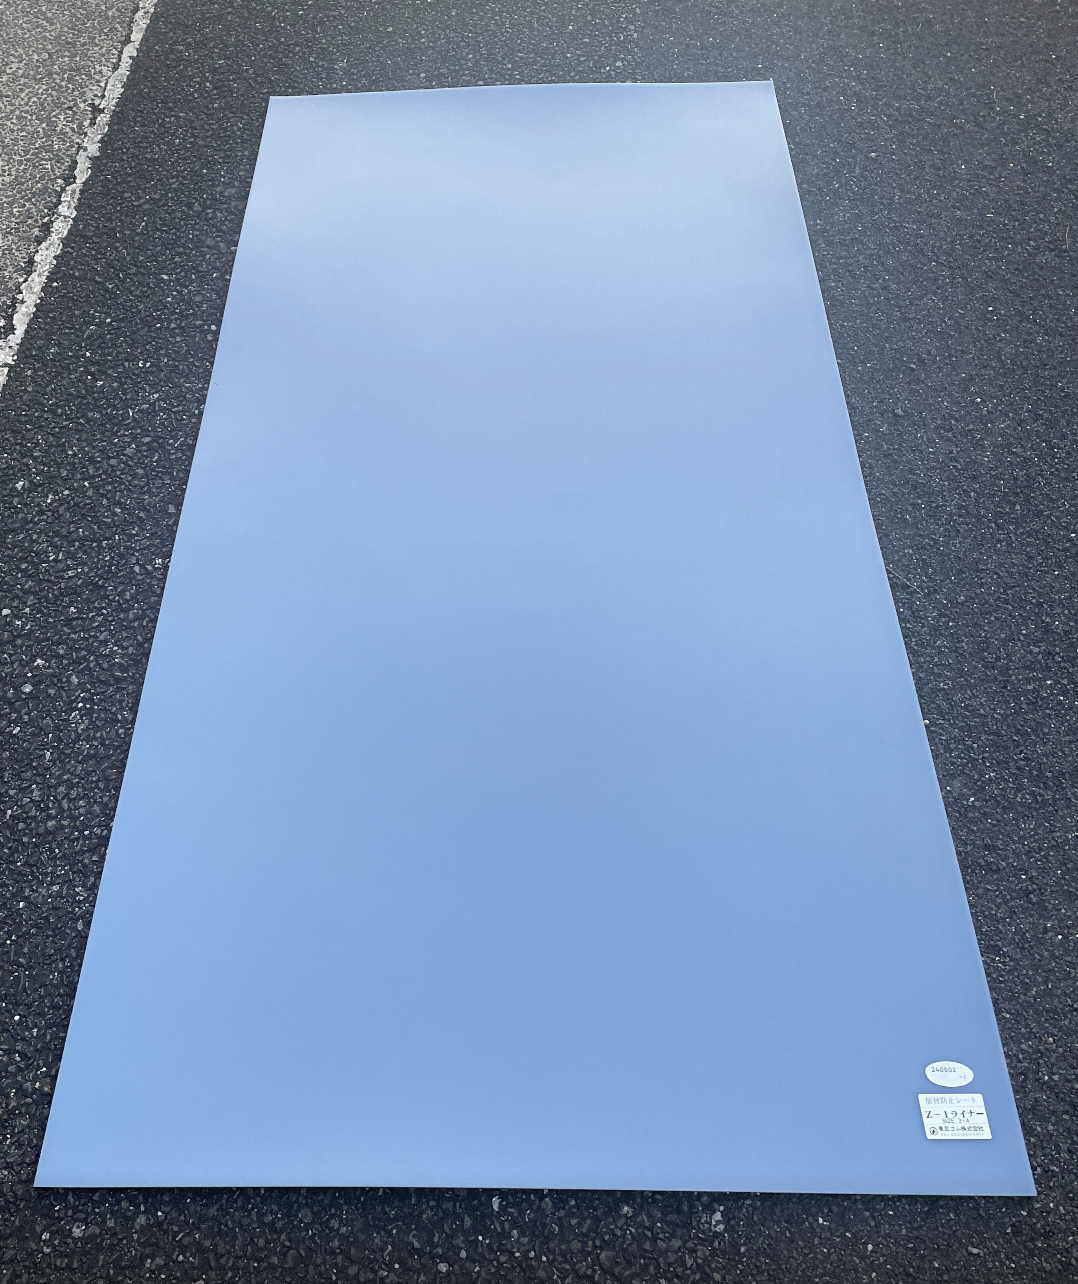
\includegraphics[width=0.25\linewidth]{fig/4_lowmusheet.png}
        \label{subfig:4_low_mu_sheet}
    }
    \caption{Experimental driving environment.}
    \label{fig:key}
\end{figure}

The target scenario is a transition from a high-$\mu$ road surface to a low-$\mu$ road surface during driving force control, as illustrated in Fig.~\ref{subfig:4_road_condition}.
In the vehicle experiments, a non-adhesive composite sheet, as shown in the figure, was used to reproduce a low-$\mu$ road surface.
By spraying water onto the sheet, a low-friction road surface with a peak friction coefficient of approximately $\mu_\mathrm{peak} = 0.25$ can be reproduced.

The vehicle starts from a standstill on a high-$\mu$ road surface, and the estimation of $\lambda_\mathrm{peak}$ is initiated simultaneously.
After traveling $\SI{10}{m}$, the vehicle enters the low-friction sheet and travels an additional $\SI{20}{m}$.
The driving force command is maintained at a constant value of $900$ N.
This value can be achieved on the high-$\mu$ road surface but exceeds the physically attainable driving force on the low-$\mu$ road surface, thereby causing wheel slip.

The pole of the wheel-speed control system for driving force control was set to $\omega_\mathrm{n} = -20$ rad/s, and the integral gain of the outer loop was set to $K_\mathrm{i} = 0.1$.
Furthermore, the cutoff frequency of the low-pass filter (LPF) applied to $\hat{\lambda}_\mathrm{peak}$ was set to $\omega_c = 10$ rad/s.


\subsection{Experimental Results}
\begin{figure}[tb]
    \centering
        \subfloat[Conventional method.]{
        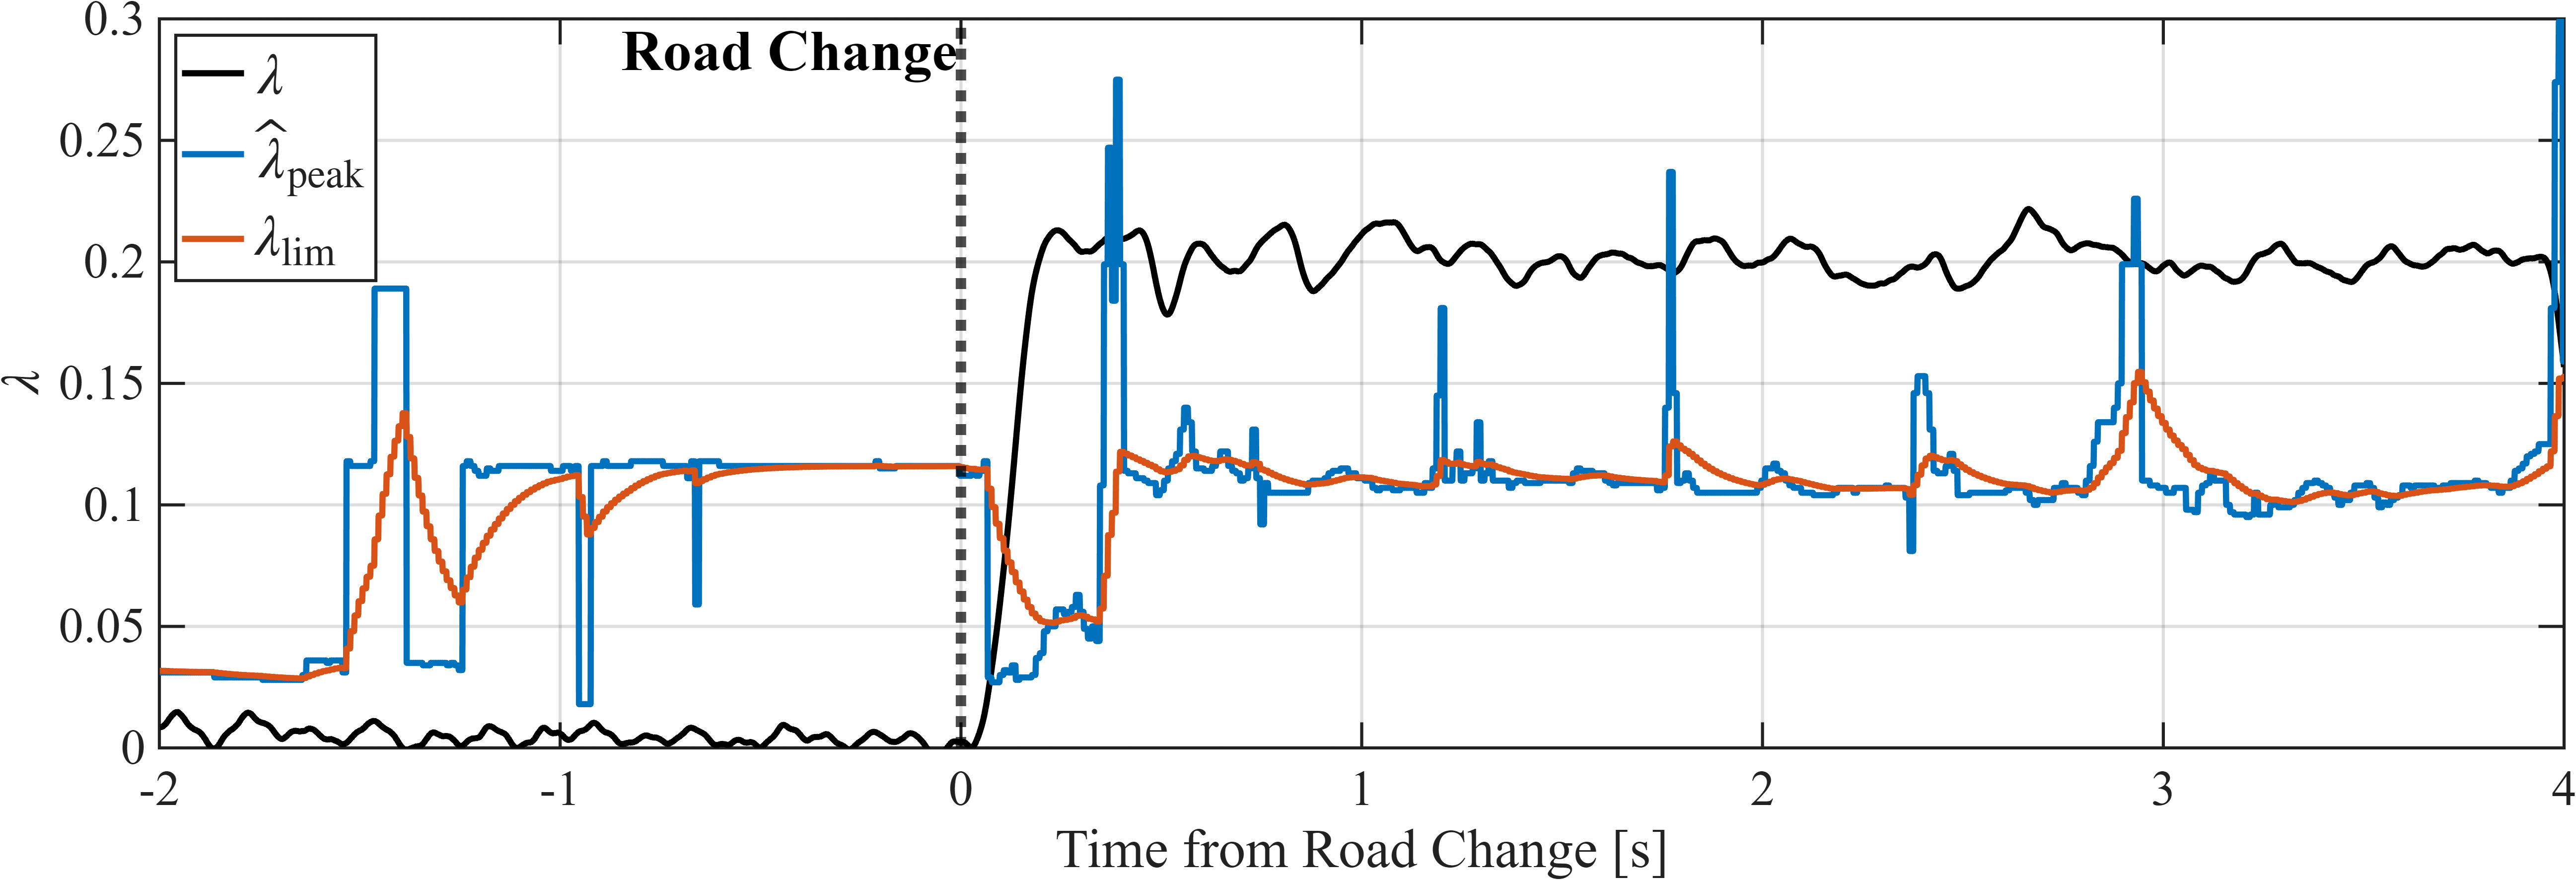
\includegraphics[width=0.8\linewidth]{fig/SlipRatioComparison_Data053.png}
        \label{subfig:4_result_lambda_old}
    }
    
    \vspace{2mm}

    \subfloat[Proposed method.]{
        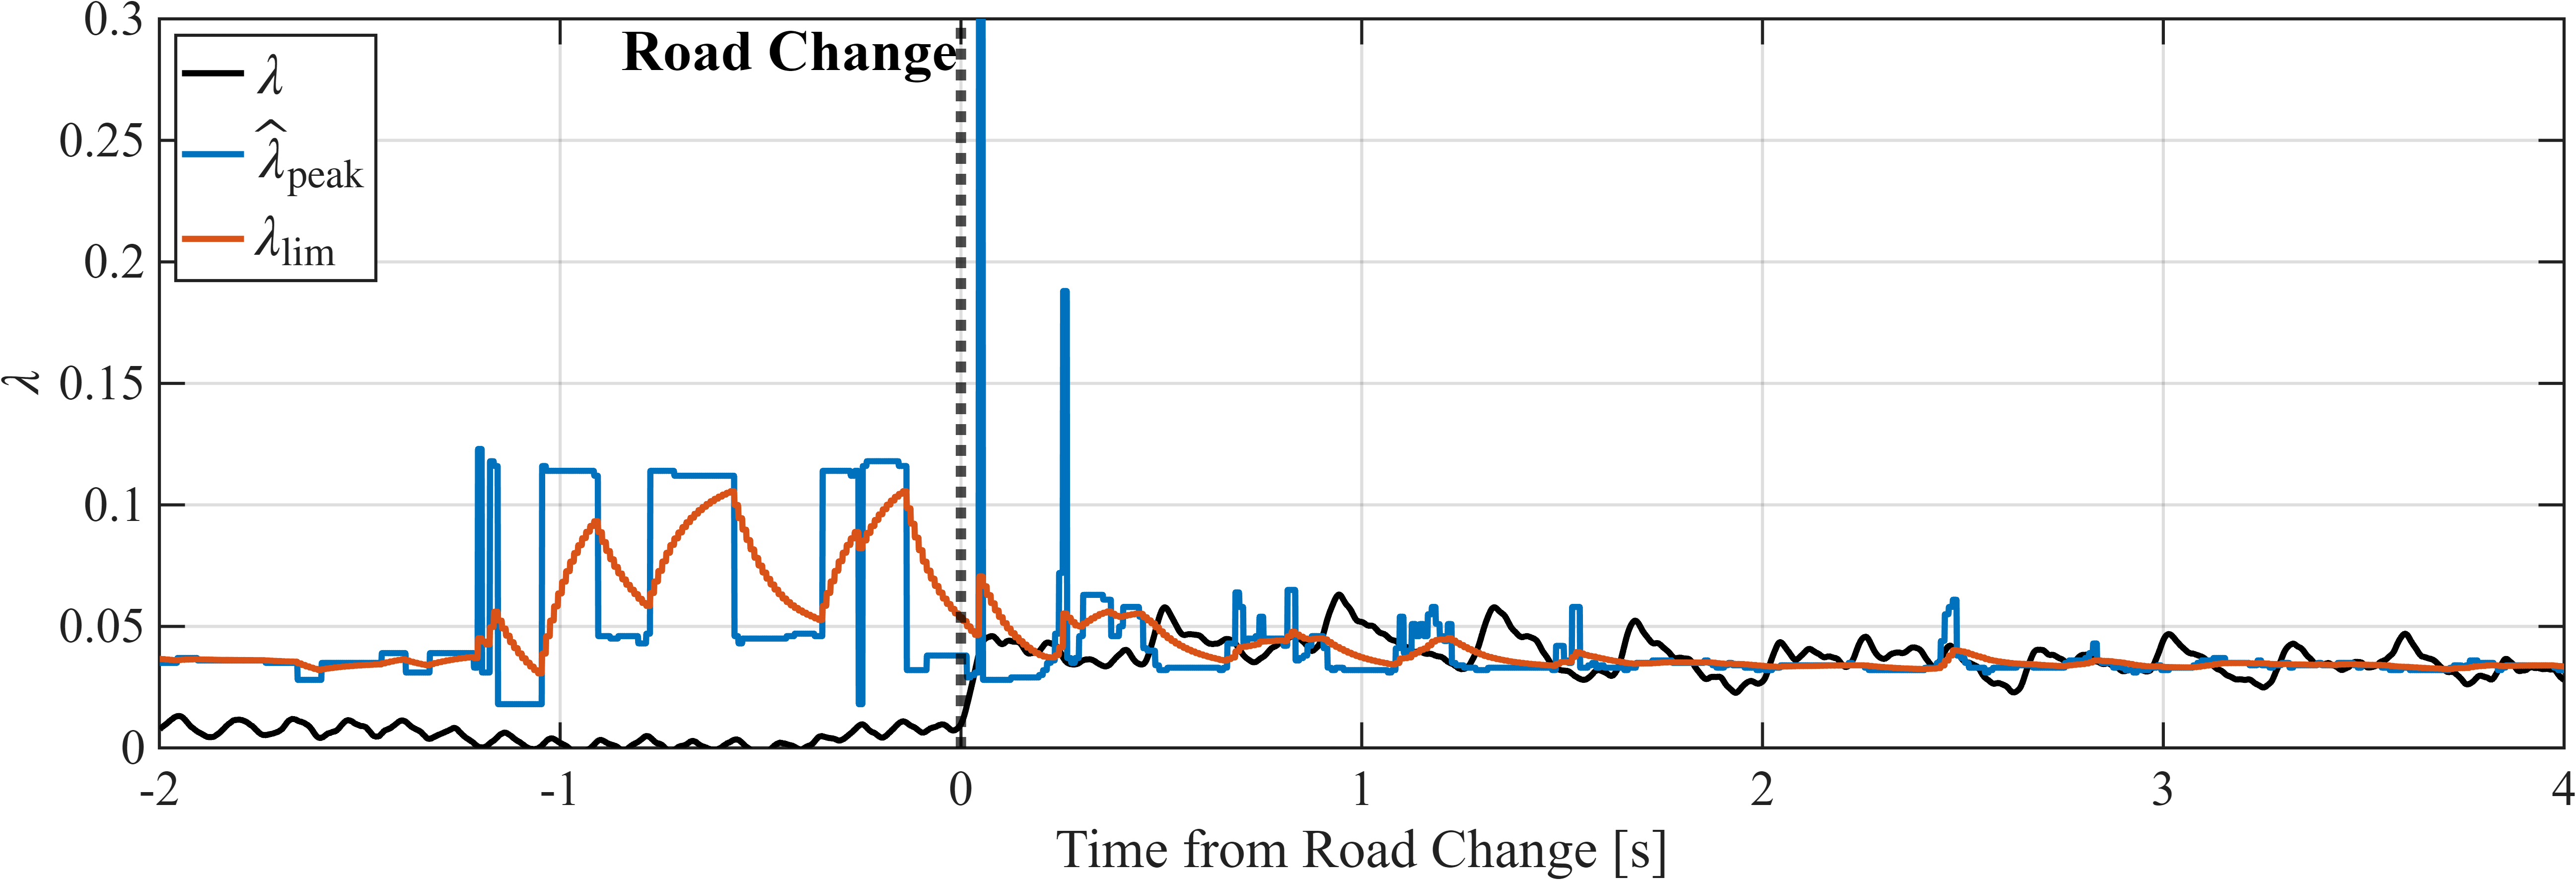
\includegraphics[width=0.8\linewidth]{fig/SlipRatioComparison_Data077.png}
        \label{subfig:4_result_lambda_prop}
    }

    \vspace{2mm}

    \subfloat[Zoom of proposed method.]{
        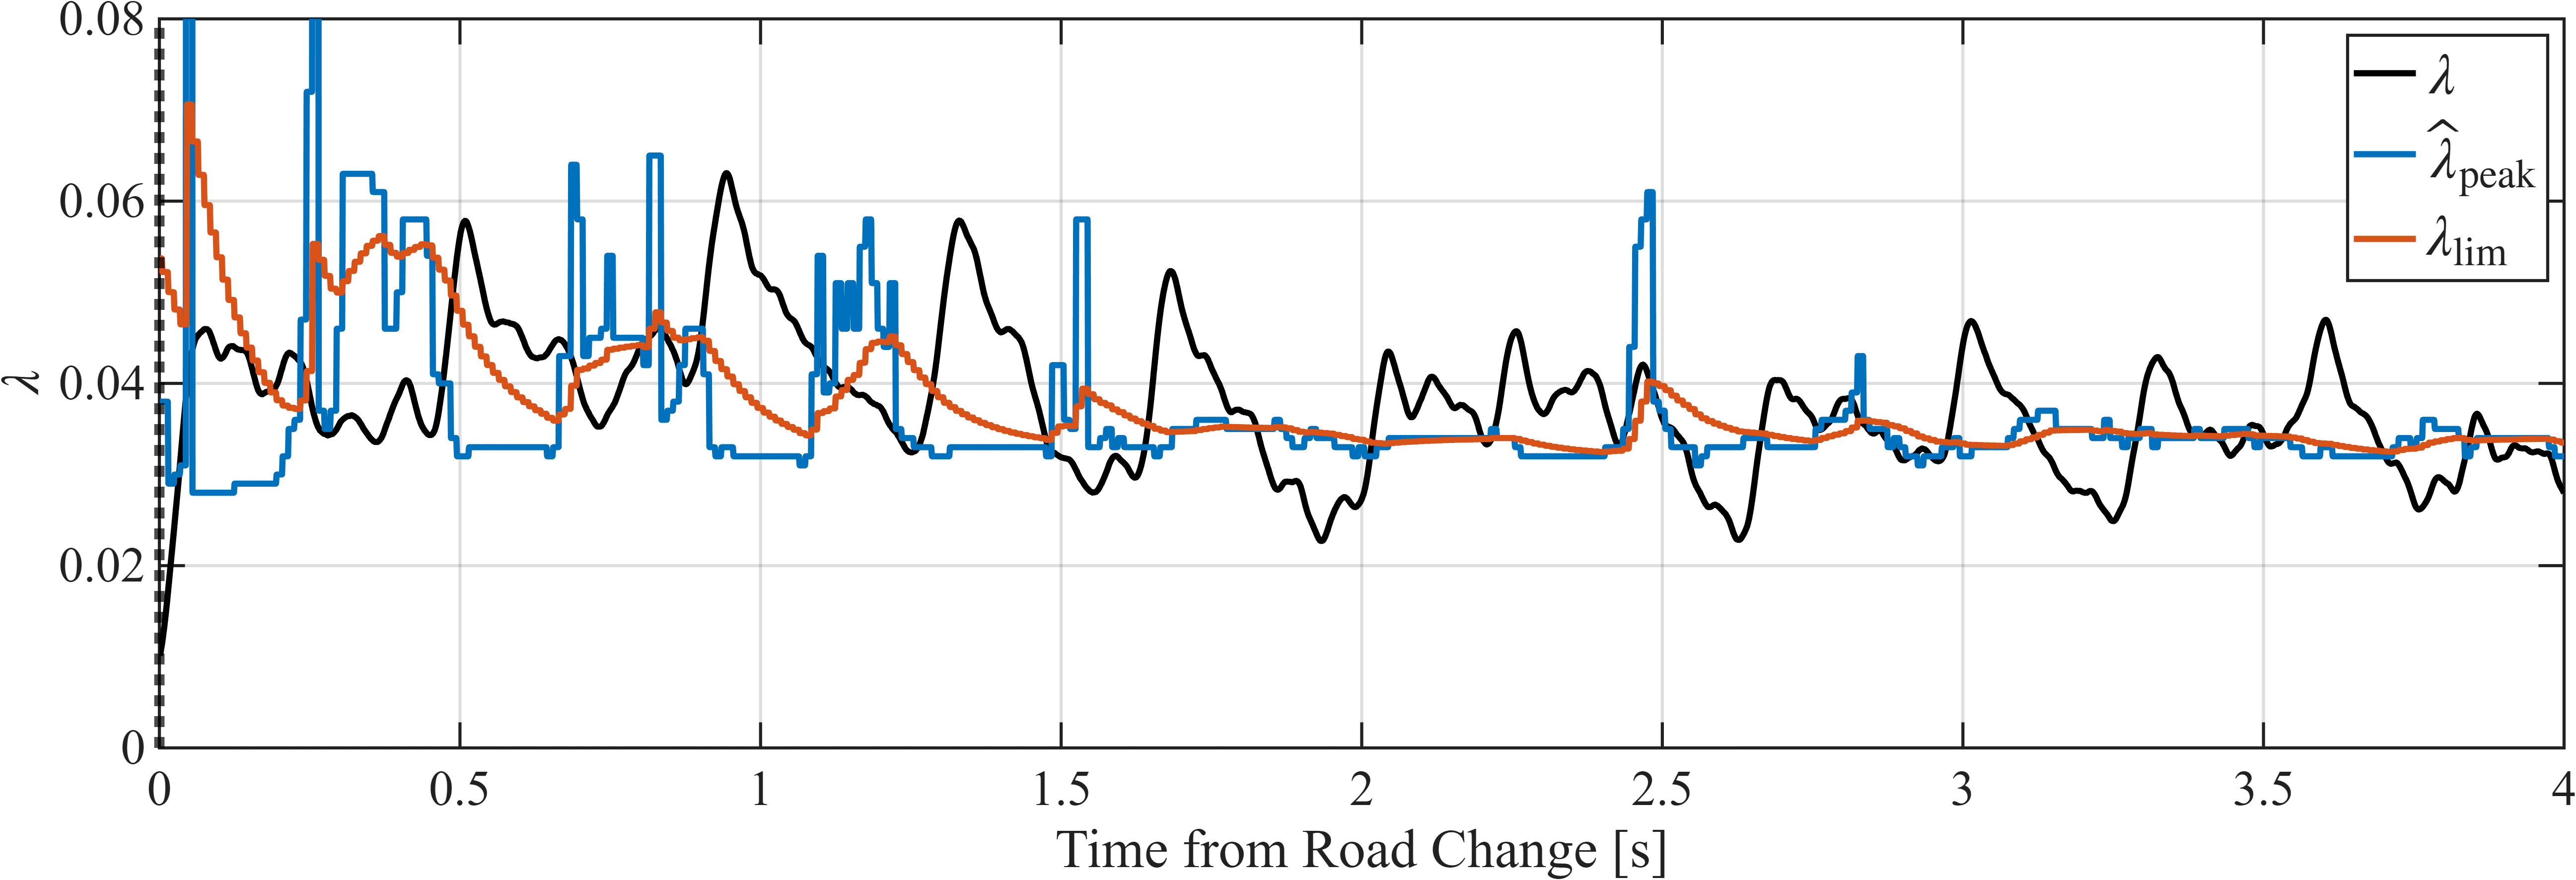
\includegraphics[width=0.8\linewidth]{fig/SlipRatioComparison_Data077_zoom.png}
        \label{subfig:4_result_lambda_prop_zoom}
    }


    \caption{Comparison of the proposed and conventional methods.}
    \label{fig:4_result_lambda}
\end{figure}
Two driving experiments were conducted: one using the proposed method and the other using a conventional method in which the slip ratio limiter was fixed at $\lambda_\mathrm{lim} = 0.2$.
The time histories of the slip ratio limiter and the measured slip ratio for both methods are shown in Fig.~\ref{fig:4_result_lambda}.
The time axis is set such that the road surface transition occurs at 0 s, and the data from 2 s before to 4 s after the transition are presented.

As shown in the figure, with the conventional method, the slip ratio remains at the fixed limiter value after the transition to the low-$\mu$ road surface, resulting in a high-slip condition.
In contrast, the proposed method prevents the slip ratio from reaching such a high value after the transition and maintains it within a low-slip region.

\begin{figure}[tb]
  \centering
  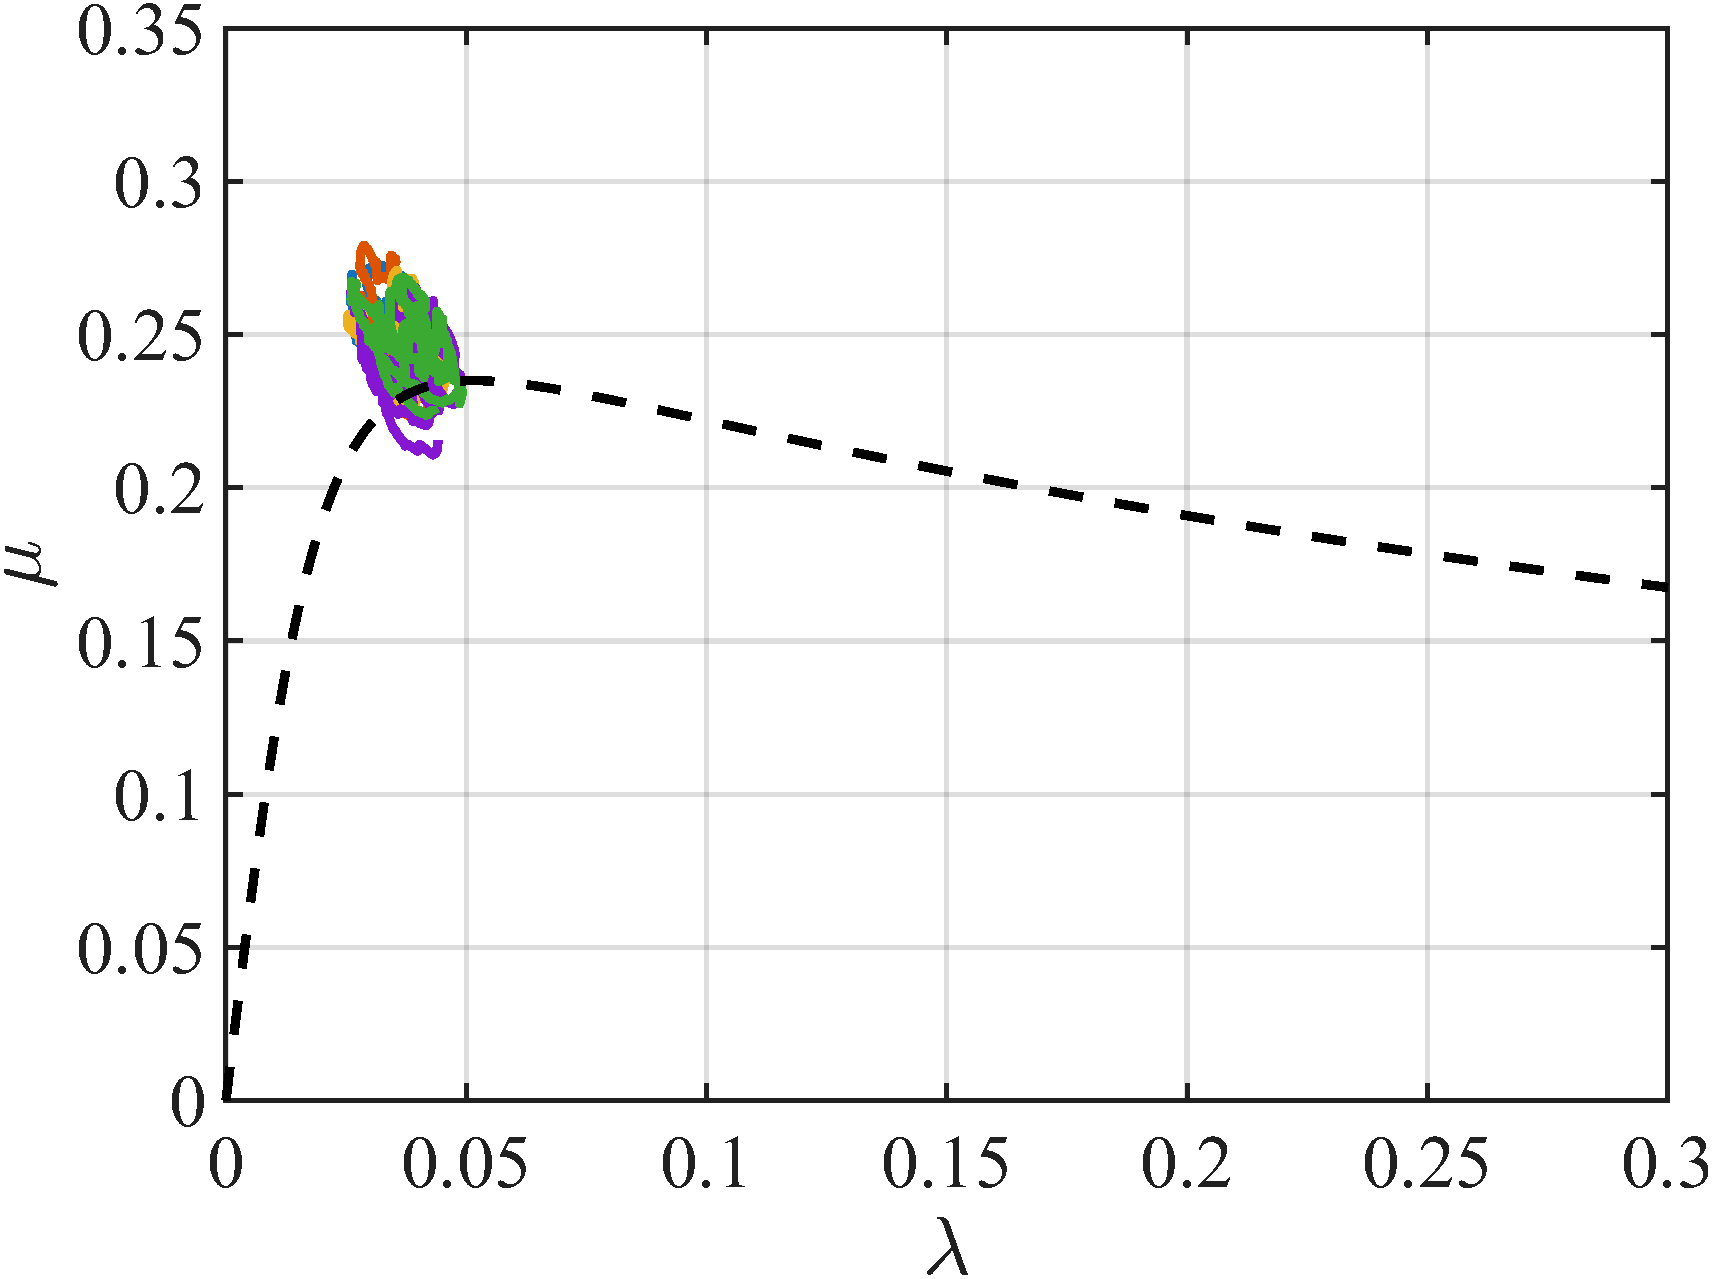
\includegraphics[width=0.7\linewidth]{fig/4_result_mu_lambda.pdf}
  \caption{Measured $\mu$--$\lambda$ plot.}
  \label{fig:4_result_mu_lambda}
\end{figure}

Figure~\ref{fig:4_result_mu_lambda} shows the measured $\mu$--$\lambda$ plots obtained using the proposed method.
The results of five experiments are superimposed, and only the data points measured after entering the low-$\mu$ road surface are plotted.

The black dashed curve in the figure represents a Magic Formula curve fitted to the measurement data obtained in a previous study under the same road surface conditions.
The corresponding model parameters were $B = 28.9114$, $C = 1.9078$, $D = 0.2350$, and $E = 0.8100$ \cite{mizuguchi2026}.

These results demonstrate that the proposed method can maintain the slip ratio near the peak point of the fitted road-surface characteristic curve.


\section{Conclusion}

This paper proposed an algorithm for estimating the optimal slip ratio $\lambda_\mathrm{peak}$ based on online estimation of the $\mu$--$\lambda$ curve using a multilayer perceptron (MLP).
The validity of the estimation results was then experimentally verified through driving force control.

Future work includes quantitatively evaluating the differences in acceleration performance resulting from different slip ratio limiters.
Furthermore, although the proposed method was experimentally validated on a single low-$\mu$ road surface in this study, its generalization performance under multiple road surface conditions with different friction characteristics remains to be investigated.



% \section*{Acknowledgment}

% The preferred spelling of the word ``acknowledgment'' in America is without 
% an ``e'' after the ``g''. Avoid the stilted expression ``one of us (R. B. 
% G.) thanks $\ldots$''. Instead, try ``R. B. G. thanks$\ldots$''. Put sponsor 
% acknowledgments in the unnumbered footnote on the first page.


\bibliographystyle{IEEEtran} 
\bibliography{reference}

\end{document}
